\documentclass[12pt,a4paper]{article}
\usepackage[utf8]{inputenc}
\usepackage[utf8]{vietnam} %Bien dich duoc tieng Viet
\usepackage{amsmath,amsfonts,amssymb} %Font toan
\usepackage{xfrac}
\usepackage{type1cm}
\usepackage{graphicx}
%\usepackage{subfigure}
\usepackage{subfig}
\graphicspath{ {images/} }
\usepackage{multirow}
\usepackage{multicol}
\usepackage{array}
\usepackage{comment}
\usepackage{enumerate}
\usepackage[unicode]{hyperref}
\usepackage{indentfirst}
\usepackage{color}
\usepackage[left=1.5cm,right=1.5cm,top=2cm,bottom=2cm]{geometry}
\usepackage[american,cuteinductors,smartlabels]{circuitikz}
\usetikzlibrary{arrows}
\usepackage{tikz}
\usetikzlibrary{calc,patterns,angles,quotes}
\usetikzlibrary{arrows, decorations.markings, calc, fadings, decorations.pathreplacing, patterns, decorations.pathmorphing, positioning}	
%\tikzstyle{every path}=[line width=1.2pt]
%\title{\textbf{Giải bài tập Thiết kế hệ thống điện}}
\title{\textbf{Bài tập ôn thi giữa kỳ\vspace{.4cm}\\Môn học Thiết kế hệ thống điện}}
\author{SVTH: Thi Minh Nhựt -- Email: thiminhnhut@gmail.com}
%\date{Ngày 05 tháng 10 năm 2016}
\date{Thời gian: \today}

\begin{document}
\pagenumbering{gobble}
\maketitle
\everymath{\displaystyle}
%%
%%
\tableofcontents
%\listoffigures
%\listoftables
\newpage
\pagenumbering{arabic}
\newcommand{\unit}[1]{~#1} % Sau số có cách khoảng đơn vị
\newcommand{\unitp}[1]{~\left({#1}\right)} %Cặp dấu ngoặc của đơn vị
\newcommand{\pfm}[1]{\left({#1}\right)} %Cặp dấu ngoặc trong công thức
\renewcommand{\arraystretch}{1.3} 																% Một số lệnh LaTeX được định nghĩa lại vào tạo mới
\section{Các thông số đường dây truyền tải trên không}
\subsection{Điện trở của đường dây truyền tải trên không}
\begin{itemize}
\item Với dây dẫn có chiều dài $l \unitp{m}$, tiết diện dây dẫn $A \unitp{m^2}$, điện trở suất $\rho \unitp{\Omega m}$, điện trở $R$ được xác định: $$ R = \dfrac{\rho l}{A} \unitp{\Omega}$$.
\item Giá trị của điện trở suất $\rho \unitp{\Omega m}$ ở $20^0C$:
\begin{table}[!h]
\begin{center}
\begin{tabular}{|l|c|}\hline
Dây đồng thường, dẫn điện $100\%$ & $\rho = 1.724 \times 10^{-8} $ \\ \hline
Dây đồng kéo cứng, dẫn điện $97.3\%$ & $\rho = 1.78 \times 10^{-8} $ \\  \hline
Dây đồng nhôm, dẫn điện $61\%$ & $\rho = 2.86 \times 10^{-8} $ \\ \hline
Dây sắt hoặc dây thép & $\rho = 12.2 \times 10^{-8} $ \\ \hline
\end{tabular}
\end{center}
\caption{Giá trị điện trở suất $\rho$ của một số kim loại ở $t^0 = 20^0C$} \label{Tab:gia-tri-dien-tro-suat}
\end{table}
\item  Với $R_0$ là điện trở ở $20^0C$, điện trở thay đổi theo nhiệt độ $t$ được xác định bằng công thức: $$R = R_0 \left[{1 + \alpha \left({t - 20}\right)}\right]$$
\begin{table}[!h]
\begin{center}
\begin{tabular}{|l|c|c|}\hline
Kim loại & Điện trở suất $\unitp{\Omega m}$ & Hệ số nhiệt điện trở $\alpha \unitp{^0C^{-1}}$ \\ \hline
Nhôm & $2.83 \times 10^{-8}$ & $0.0039$ \\ \hline
Đồng cứng & $1.77 \times 10^{-8}$ & $0.00382$ \\ \hline
Đồng thường & $1.72 \times 10^{-8}$ & $0.00393$ \\ \hline
Sắt & $10.00 \times 10^{-8}$ & $0.0050$ \\ \hline
Thép & $(12 \div 88) \times 10^{-8}$ & $0.001 \div 0.005$ \\ \hline
Bạc & $1.53 \times 10^{-8}$ & $0.0038$ \\ \hline
Đồng thau & $(6.4 \div 8.4) \times 10^{-8}$ & $0.0020$ \\ \hline
\end{tabular}
\end{center}
\caption{Hệ số nhiệt điện trở $\alpha$ và điện trở suất $\rho$ của một số kim loại ở $t^0 = 20^0C$} \label{Tab:he-so-nhiet-dien-tro-gia-tri-dien-tro-suat}
\end{table}
\end{itemize}
\newpage
\subsection{Xác định khoảng cách trung bình hình học và bán kính trung bình hình học giữa các dây dẫn}\label{Sec:Dm-Ds}
\begin{enumerate}[\it a.]
\item \textit{Mạch một pha có 2 dây dẫn song song, mỗi dây gồm 1 sợi}
\begin{figure}[!h]
\begin{center}
\begin{tikzpicture}
\draw (0,0) circle (.5);
\draw[dashed] (0,1) -- (0,-1.5);
\draw[dashed] (0,0) -- (-.5,.5) -- (-1.5,.5);
\draw (-1,.7) node{$r$};
\draw[-triangle 90, dashed] (2,-1) -- (0,-1);
\draw[-triangle 90, dashed] (2,-1) -- (4,-1);
\draw (2,-.7) node{$D$};
\draw (4,0) circle (.5);
\draw[dashed] (4,0) -- (4.5,.5) -- (5.5,.5);
\draw (5,.7) node{$r$};
\draw[dashed] (4,1) -- (4,-1.5);
\end{tikzpicture}
\end{center}
\caption{Mạch một pha có hai dây dẫn song song song} \label{Fig:mach-mot-pha-2-day-song-song}
\end{figure}
\subparagraph{Giả thiết} Cho đường dây một pha gồm 2 dây dẫn song song, đặt cách nhau một khoảng $D$, mỗi dây dẫn có bán kính là $r$ được mô tả trên hình \ref{Fig:mach-mot-pha-2-day-song-song}.
\subparagraph{Kết quả}
\begin{itemize}
\item Khoảng cách trung bình hình học -- GMD: $D_m = D$.
\item Bán kính trung bình hình học -- GMR: $D_s = r^\prime = re^{-0.25}$.
\end{itemize}
\item \textit{Đường dây một pha mạch kép}
\begin{figure}[!h]
\begin{center}
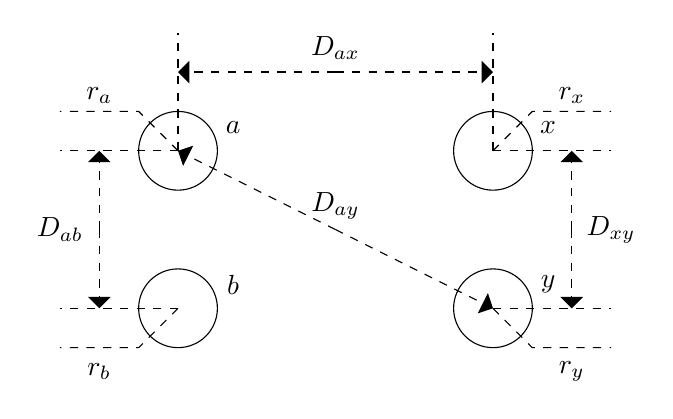
\begin{tikzpicture}
\draw (0,0) circle (.5); \draw (0.7,0.3) node{$a$}; \draw[dashed] (0,0) -- (0,1.5); \draw[dashed] (0,0) -- (-1.5,0); 
\draw (4,0) circle (.5); \draw (4.7,0.3) node{$x$}; \draw[dashed] (4,0) -- (4,1.5);  \draw[dashed] (4,0) -- (5.5,0); 
\draw (0,-2) circle (.5); \draw (0.7,-1.7) node{$b$}; \draw[dashed] (0,-2) -- (-1.5,-2); 
\draw (4,-2) circle (.5);	\draw (4.7,-1.7) node{$y$}; \draw[dashed] (4,-2) -- (5.5,-2); 

\draw[-triangle 90, dashed] (2,1) -- (0,1);
\draw[-triangle 90, dashed] (2,1) -- (4,1);
\draw (2,1.3) node{$D_{ax}$};

\draw[-triangle 90, dashed] (-1,-1) -- (-1,0);
\draw[-triangle 90, dashed] (-1,-1) -- (-1,-2);
\draw (-1.5,-1) node{$D_{ab}$};

\draw[-triangle 90, dashed] (5,-1) -- (5,0);
\draw[-triangle 90, dashed] (5,-1) -- (5,-2);
\draw (5.5,-1) node{$D_{xy}$};

\draw[-triangle 90, dashed] (2,-1) -- (0,0);
\draw[-triangle 90, dashed] (2,-1) -- (4,-2);
\draw (2,-.7) node{$D_{ay}$};

\draw[dashed] (0,0) -- (-.5,.5) -- (-1.5,.5);
\draw (-1,.7) node{$r_a$};

\draw[dashed] (0,-2) -- (-.5,-2.5) -- (-1.5,-2.5);
\draw (-1,-2.8) node{$r_b$};

\draw[dashed] (4,0) -- (4.5,.5) -- (5.5,.5);
\draw (5,.7) node{$r_x$};

\draw[dashed] (4,-2) -- (4.5,-2.5) -- (5.5,-2.5);
\draw (5,-2.8) node{$r_y$};
\end{tikzpicture}
\end{center}
\caption{Đường dây một pha mạch kép} \label{Fig:mach-mot-pha-2-day-song-song-lo-kep}
\end{figure}
\subparagraph{Giả thiết} Cho đường dây một pha gồm 2 dây dẫn song song với các kích thước và khoảng cách được mô tả trên hình \ref{Fig:mach-mot-pha-2-day-song-song-lo-kep}.
\subparagraph{Kết quả}
\begin{itemize}
\item Khoảng cách trung bình hình học -- GMD: $D_m = \sqrt[4]{D_{ax}D_{ay}D_{bx}D_{by}}$
\item Bán kính trung bình hình học -- GMR:
\begin{itemize}
\item Dây dẫn $ab$: $D_s = \sqrt[4]{r_a^{\prime} r_b^{\prime} D_{ab} D_{ba}}$%, với $r_a^\prime = r_a  e^{-0.25}$ và $r_b^\prime = r_b  e^{-0.25}$.
\item Dây dẫn $xy$: $D_s = \sqrt[4]{r_x^{\prime} r_ y^{\prime} D_{xy} D_{yx}}$%, , với $r_x^\prime = r_x e^{-0.25}$ và $r_y^\prime = r_y e^{-0.25}$.
\item[$\ast$] Các giá trị $r^\prime$ có được bằng cách tra bảng \ref{Tab:GMD-day-dan-ben-nhieu-soi} trang \pageref{Tab:GMD-day-dan-ben-nhieu-soi}.
\end{itemize}
\end{itemize}
\newpage
\item \textit{Dây dẫn bện nhiều sợi}

Với dây dẫn bện nhiều sợi, khoảng cách trung bình hình học -- GMD được cho trong bảng \ref{Tab:GMD-day-dan-ben-nhieu-soi}.
\begin{table}[!h]
\begin{center}
\begin{tabular}{|c|c||c|c|}\hline
Số sợi & GMD & Số sợi & GMD \\ \hline
1 & $0.779R$ & 91 & $0.774R$ \\ \hline
7 & $ 0.726R$ & 127 & $0.776R$\\ \hline
19 & $0.758R$ & 30 (2 lớp) & $0.826R$ \\ \hline
37 & $0.768R$ & 26 (2 lớp) & $0.809R$\\ \hline
61 & $0.772R$ & 54 (3 lớp) & $0.810R$\\ \hline
\multicolumn{4}{|c|}{$R$ là bán kính ngoài của dây dẫn bện nhiều sợi}\\ \hline
\end{tabular}
\end{center}
\caption{GMD của dây dẫn nhiều sợi} \label{Tab:GMD-day-dan-ben-nhieu-soi}
\end{table}
\item \textit{Mạch ba pha lộ đơn}
\begin{figure}[!h]
\begin{center}
\begin{tikzpicture}
\draw (0,0) circle (0.5);  \draw (0,-.5) node[below]{$b$};
\draw (4,0) circle (0.5); \draw (4,-.5) node[below]{$c$};
\draw (2,3.5) circle (0.5);\draw (2,4) node[above]{$a$};
\draw[dashed] (0,0) -- (4,0) -- (2, 3.5) -- (0,0);
\draw (2, 0) node[below] {$D_{bc}$};
\draw (0.6, 1.75) node[left] {$D_{ab}$};
\draw (3.4, 1.75) node[right] {$D_{ac}$};
\end{tikzpicture}
\end{center}
\caption{Mạch ba pha lộ đơn} \label{Fig:mach-ba-lo-don}
\end{figure}
\subparagraph{Giả thiết} Cho đường dây ba pha lộ đơn như hình \ref{Fig:mach-ba-lo-don}.
\subparagraph{Kết quả}
\begin{itemize}
\item Khoảng cách trung bình hình học -- GMD: $D_m = \sqrt[3]{D_{ab}D_{bc}D_{ac}}$. \item Bán kính trung bình hình học -- GMR: $D_s = \sqrt[3]{r_{a}^\prime r_{b}^\prime r_{c}^\prime}$.
\item[$\ast$] Các giá trị $r^\prime$ có được bằng cách tra bảng \ref{Tab:GMD-day-dan-ben-nhieu-soi} trang \pageref{Tab:GMD-day-dan-ben-nhieu-soi}.
\end{itemize}

\item \textit{Mạch ba pha đường lộ kép}
\begin{figure}[!h]
\begin{center}
\begin{tikzpicture}
\draw (0,0) circle (.5); \draw (0.5, 0) node[right]{$a$};
\draw (-2,-2) circle (.5); \draw (-1.5, -2) node[right]{$b$};
\draw (0,-4) circle (.5); \draw (0.5, -4) node[right]{$c$};
\draw (6,0) circle (.5); \draw (5, 0) node[right]{$c^\prime$};
\draw (8,-2) circle (.5);  \draw (7, -2) node[right]{$b^\prime$};
\draw (6,-4) circle (.5); \draw (5, -4) node[right]{$a^\prime$};
\end{tikzpicture}
\end{center}
\caption{Mạch ba pha đảo pha trên đường dây lộ kép} \label{Fig:mach-ba-duong-day-kep}
\end{figure}
\subparagraph{Giả thiết} Cho đường dây ba pha lộ kép thực hiện đảo pha như hình \ref{Fig:mach-ba-duong-day-kep}.
\subparagraph{Kết quả}
\begin{itemize}
\item Khoảng cách trung bình hình học -- GMD: $D_m = \sqrt[3]{D_{AB}D_{BC}D_{AC}}$. Với:
	\begin{align*}
	 D_{AB} = \sqrt[4]{D_{ab} D_{ab^\prime} D_{a^\prime b} D_{a^\prime b^\prime}}; \qquad D_{BC} = \sqrt[4]{D_{bc} D_{bc^\prime} D_{b^\prime c} D_{b^\prime c^\prime}}; \quad D_{AC} = \sqrt[4]{D_{ac} D_{ac^\prime} D_{a^\prime c} D_{a^\prime c^\prime}}
	\end{align*}
\item Bán kính trung bình hình học -- GMR: $D_s = \sqrt[3]{D_{sA}  D_{sB} D_{sC}}$. Với: 
	\begin{align*}
		D_{sA}  = \sqrt{r^\prime D_{a a^\prime}}; \quad D_{sB}  = \sqrt{r^\prime D_{ b b^\prime}}; \quad D_{sC}  = \sqrt{r^\prime D_{c c^\prime}}
	\end{align*}
	\item[$\ast$] Các giá trị $r^\prime$ có được bằng cách tra bảng \ref{Tab:GMD-day-dan-ben-nhieu-soi} trang \pageref{Tab:GMD-day-dan-ben-nhieu-soi}.
\end{itemize}
\end{enumerate}
\subsection{Điện cảm và cảm kháng}
\begin{itemize}
\item Điện cảm trên $1\unit{km}$ của dây dẫn: $L_0 = 2 \times 10^{-4}\times \ln{\dfrac{D_m}{D_s}} \unitp{H/km}$.
\item Điện kháng trên $1\unit{km}$ dây dẫn: $x_0 = \omega L_0 = 2\pi f L_0 \unitp{\Omega/km}$.
\item Điện cảm trên toàn bộ đường dây có chiều dài  $l \unitp{km}$: $L = L_0 \times l$.
\item Điện kháng trên toàn bộ đường dây có chiều dài  $l \unitp{km}$: $X = x_0 \times l$.
\end{itemize}
\subsection{Điện dung, dung kháng và dung dẫn}
\begin{itemize}
\item Điện dung trên một $km$ so với trung tính:
	\begin{align*}
		C_0 =\dfrac{1}{18 \times 10^6 \times  \ln{\dfrac{D_m}{D_s}}} \unitp{F/km}
	\end{align*}
\item[$\ast$] \emph{Lưu ý:} Khi tính điện dung thì thay $r^\prime = r$ vào các công thức tính $D_s$ và $D_m$ được xác định như các công thức ở phần \ref{Sec:Dm-Ds} trang \pageref{Sec:Dm-Ds}.
\item Dung kháng trên một $km$:
	\begin{align*}
		x_0 = \dfrac{1}{\omega C_0} = \dfrac{18 \times 10^6 \times \ln{\dfrac{D_m}{D_s}} }{2\pi f} \unitp{\Omega / km}
	\end{align*}
\item Dung dẫn trên một $km$:
	\begin{align*}
		b_0 = \omega C_0 = \dfrac{2\pi f}{18 \times 10^6 \times  \ln{\dfrac{D_m}{D_s}}} \unitp{\Omega^{-1}/km}
	\end{align*}
\item Điện dung trên toàn bộ đường dây có chiều dài  $l \unitp{km}$: $C = C_0 \times l$.
\item Dung kháng trên toàn bộ đường dây có chiều dài  $l \unitp{km}$: $X = x_0 \times l$.
\item Dung dẫn trên toàn bộ đường dây có chiều dài  $l \unitp{km}$: $B = b_0 \times l$.
\end{itemize}
\subsection{Một số đơn vị dùng đo kích thước và chiều dài dây dẫn}
\begin{table}[!h]
\begin{center}
\begin{tabular}{|l|l|}\hline
\multicolumn{2}{|c|}{$1 \unit{mil} = 10^{-3} \unit{inch} = 2.54 \times 10^{-3} \unit{inch}$} \\ \hline
$1 \unit{inch} = 2.54 \unit{cm}$ & $1 \unit{cm} = 0.3937 \unit{inch} = 393.7 \unit{mil}$\\ \hline
$1 \unit{mile} = 1609 \unit{m} = 1.609 \unit{km}$ & $1 \unit{km} = 0.6214 \unit{mile}$ \\ \hline
$1 \unit{foot} = 30.48 \unit{cm} = 3.048 \unit{dm}$ & $1 \unit{m} = 3.281 \unit{foot}$ \\ \hline
$1 \unit{foot} = 12 \unit{inch}$ & \\ \hline
$1 \unit{CM} = 5.067 \unit{mm^2}$ & $1 \unit{MCM} = 10^3 \unit{CM}$\\ \hline
\end{tabular}
\end{center}
\caption{Đơn vị thường dùng để đo kích thước dây dẫn}\label{Tab:don-vi-do-kich-thuoc-day-dan}
\end{table}
\subsection{Bài tập về các thông số đường dây truyền tải trên không}
\begin{enumerate}
\item \label{Ex-1} Tính điện cảm của mỗi $km$ đường dây truyền tải trên không một pha, dây dẫn bằng đồng, đặt cách nhau $1m$ và đường kính $1\unit{cm}$.
\subparagraph{Bài giải bài tập \ref{Ex-1}}
\begin{itemize}
\item Xác định $D_m$ và $D_s$:
	\begin{align*}
		D_m & = D = 1 \unit{m} = 100 \unit{cm}\\
		D_s & = r^{\prime} = r \times e^{-0.25} = \dfrac{1}{2} \times e^{-0.25} = 0.389 \unit{cm}
	\end{align*}
\item Nên: $L_0 = 2 \times 10^{-4} \times \ln{\dfrac{D_m}{D_s}}  =  L_0 = 2 \times 10^{-4} \times \ln{\dfrac{100}{0.389}} = 1.110 \times 10^{-3} \unitp{H/km}$ .
\end{itemize}
\item \label{Ex-2} Một đường dây một pha gồm 2 dây dẫn $a, a^\prime$ song song và dây dẫn $b, b^\prime$ tạo đường dây về. Khoảng cách được cho trên hình \ref{Fig:bai-tap-2}. Tính điện cảm của đường dây (đi và về) trên mỗi $km$, biết đường kính của mỗi dây làm $2.6\unit{cm}$.
\begin{figure}[!h]
\begin{center}
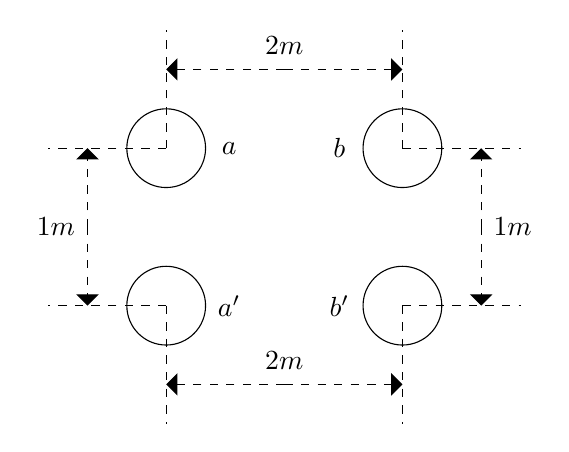
\begin{tikzpicture}
\draw (0,0) circle (.5); \draw[dashed] (0,0) -- (0,1.5); \draw[dashed] (0,0) -- (-1.5,0); \draw (0.8, 0) node{$a$};
\draw (3,0) circle (.5); \draw[dashed] (3,0) -- (3,1.5); \draw[dashed] (3,0) -- (4.5,0); \draw (2.2, 0) node{$b$};
\draw (0,-2) circle (.5); \draw[dashed] (0,-2) -- (0,-3.5); \draw[dashed] (0,-2) -- (-1.5,-2);  \draw (0.8, -2) node{$a^\prime$};
\draw (3,-2) circle (.5);  \draw[dashed] (3,-2) -- (3,-3.5); \draw[dashed] (3,-2) -- (4.5,-2);\draw (2.2, -2) node{$b^\prime$};
\draw[dashed, -triangle 90] (1.5,1) -- (0,1); \draw[dashed, -triangle 90] (1.5,1) -- (3,1); \draw (1.5,1.3) node{$2m$};
\draw[dashed, -triangle 90] (1.5,-3) -- (0,-3); \draw[dashed, -triangle 90] (1.5,-3) -- (3,-3); \draw (1.5,-2.7) node{$2m$};

\draw[dashed, -triangle 90] (-1,-1) -- (-1,0); \draw[dashed, -triangle 90] (-1,-1) -- (-1,-2); \draw (-1.4,-1) node{$1m$};
\draw[dashed, -triangle 90] (4,-1) -- (4,0); \draw[dashed, -triangle 90] (4,-1) -- (4,-2); \draw (4.4,-1) node{$1m$};
\end{tikzpicture}
\end{center}
\caption{Sơ đồ minh họa cho bài tập \ref{Ex-2}} \label{Fig:bai-tap-2}
\end{figure}

\subparagraph{Bài giải bài tập \ref{Ex-2}}
\begin{itemize}
	\item Bán kính dây dẫn $r_a = r_{a^\prime} = r_b = r_{b^\prime} = r = \dfrac{2.6}{2} = 1.3 \unit{cm} = 1.3 \times 10^{-2} \unit{m}$.
	\item Khoảng cách: $D_{a b^\prime } = D_{a^\prime b} = \sqrt{1^2 + 2^2 } = \sqrt{5} \unit{m}$.
	\item Xác định $D_m$ và $D_s$:
	\begin{align*}
		D_m & = \sqrt[4]{D_{ab} D_{ab^\prime}D_{a^\prime b} D_{a^\prime b^\prime}} = \sqrt[4]{2 \times \sqrt{5} \times \sqrt{5} \times 2} =2.115 \unit{m} \\
		D_{s_{aa^{\prime}}} & = \sqrt[4]{r_a^\prime r_{a^\prime}^\prime D_{a a^\prime} D_{a a^\prime}} = \sqrt[4]{r_a e^{-0.25} r_{a^\prime} e^{-0.25} D_{a a^\prime} D_{a a^\prime}} \\
		& = \sqrt{re^{-0.25} D_{a a^\prime}} = \sqrt{1.3 \times 10^{-2} \times e^{-0.25} \times 1} =0.101 \unit{m} \\
		D_{s_{bb^{\prime}}} & = \sqrt[4]{r_b^\prime r_{b^\prime}^\prime D_{b b^\prime} D_{b b^\prime}} = \sqrt[4]{r_b e^{-0.25} r_{b^\prime} e^{-0.25} D_{b b^\prime} D_{b b^\prime}} \\
		& = \sqrt{re^{-0.25} D_{b b^\prime}} = \sqrt{1.3 \times 10^{-2} \times e^{-0.25} \times 1} =0.101 \unit{m}
	\end{align*}
\item Xác định của đường dây đi và về trên mỗi $km$:
	\begin{align*}
		L_{0_{a a^\prime }} & = 2 \times 10^{-4} \times \ln{\dfrac{D_m}{D_{s_{a a^\prime}}}} = 2 \times 10^{-4} \times \ln{\dfrac{2.115}{0.101}} = 6.083 \times 10^{-4} \unitp{H/km}\\
		L_{0_{b b^\prime }} & = 2 \times 10^{-4} \times \ln{\dfrac{D_m}{D_{s_{b b^\prime}}}} = 2 \times 10^{-4} \times \ln{\dfrac{2.115}{0.101}} = 6.083 \times 10^{-4} \unitp{H/km}
	\end{align*}
\end{itemize}

\item \label{Ex-3} Một đường dây truyền tải trên không 3 pha, đường kính mỗi dây là $1.8 \unit{cm}$ và được bố trí như hình \ref{Fig:bai-tap-3}. Tải cân bằng và dây có hoán đổi vị trí. Tìm điện cảm của đường dây trên từng $km$ mỗi pha.
\begin{figure}[!h]
\begin{center}
\begin{tikzpicture}
\draw (0,0) circle (.5); \draw (0,-.5) node[below] {$b$};
\draw (5,0) circle (.5); \draw (5,-.5) node[below] {$c$};
\draw (1.5,3) circle (.5); \draw (1.5,3.5) node[above] {$a$};

\draw[dashed] (0,0) -- (5,0) -- (1.5,3) -- (0,0);
\draw (2.5,0) node[below] {$9m$};
\draw (3.8,1.5) node[right] {$6m$};
\draw (-.3,1.5) node[right] {$4m$};
\end{tikzpicture}
\end{center}
\caption{Sơ đồ minh họa cho bài tập \ref{Ex-3}} \label{Fig:bai-tap-3}
\end{figure}
\subparagraph{Bài giải bài tập \ref{Ex-3}}
\begin{itemize}
	\item Ta có: bán kính dây dẫn $r = \dfrac{1.8}{2} = 0.9 \unit{cm} = 9 \times 10^{-3} \unit{m}$.
	\item Suy ra: $r_a^\prime = r_b^\prime = r_c^\prime = r e^{-0.25} = 9 \times 10^{-3} \times e^{-0.25} = 7 \times 10^{-3} \unit{m}$.
	\item Xác định $D_m$ và $D_s$:
		\begin{align*}
			D_m & = \sqrt[3]{D_{ab} D_{bc} D_{ac}} = \sqrt[3]{4 \times 9 \times 6} = 6 \unit{m}\\
			D_s & = \sqrt[3]{r_{a}^\prime r_{b}^\prime r_{c}^\prime} = \sqrt[3]{7 \times 10^{-3} \times 7 \times 10^{-3} \times 7 \times 10^{-3}} = 7 \times 10^{-3} \unit{m}
		\end{align*}
		\item Điện cảm trên mỗi $km$ của mỗi pha:
		\begin{align*}
		L_0 = 2 \times 10^{-4} \times \ln{\dfrac{D_m}{D_s}} = 2 \times 10^{-4} \times \ln{\dfrac{6}{7 \times 10^{-3}}} = 1.35 \times 10^{-3} \unitp{H/km}
	\end{align*}
\end{itemize}

\item \label{Ex-4} Đường dây 3 pha mạch kép, gồm các dây dẫn $a, a^\prime, b, b^\prime$ và $c, c^\prime$ tương ứng $a, b, c$ như hình \ref{Fig:bai-tap-3}. Mỗi dây dẫn cách nhau $1m$, đường kính mỗi dây làm $2cm$. Tính điện cảm của đường dây mạch kép trên mỗi $km$ từng pha và điện kháng mỗi pha trên mỗi $km$ đường dây với tần số $50 \unit{Hz}$.
\begin{figure}[!h]
\begin{center}
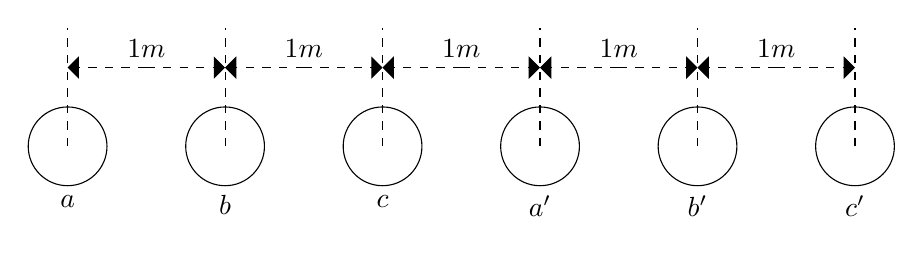
\begin{tikzpicture}
\draw (0,0) circle (.5); \draw[dashed] (0,0) -- (0,1.5); \draw (0,-0.5) node[below]{$a$};
\draw (2,0) circle (.5); \draw[dashed] (2,0) -- (2,1.5); \draw (2,-0.5) node[below]{$b$};
\draw (4,0) circle (.5); \draw[dashed] (4,0) -- (4,1.5); \draw (4,-0.5) node[below]{$c$};
\draw (6,0) circle (.5); \draw[dashed] (6,0) -- (6,1.5); \draw (6,-0.5) node[below]{$a^\prime$};
\draw (8,0) circle (.5); \draw[dashed] (8,0) -- (8,1.5); \draw (8,-0.5) node[below]{$b^\prime$};
\draw (10,0) circle (.5); \draw[dashed] (10,0) -- (10,1.5); \draw (10,-0.5) node[below]{$c^\prime$};

\draw[dashed, -triangle 90] (1,1) -- (0,1); \draw[dashed, -triangle 90] (1,1) -- (2,1);\draw (1,1) node[above] {$1m$};

\draw[dashed, -triangle 90] (3,1) -- (2,1); \draw[dashed, -triangle 90] (3,1) -- (4,1);\draw (3,1) node[above] {$1m$};

\draw[dashed, -triangle 90] (5,1) -- (4,1); \draw[dashed, -triangle 90] (5,1) -- (6,1);\draw (5,1) node[above] {$1m$};

\draw[dashed, -triangle 90] (7,1) -- (6,1); \draw[dashed, -triangle 90] (7,1) -- (8,1);\draw (7,1) node[above] {$1m$};

\draw[dashed, -triangle 90] (9,1) -- (8,1); \draw[dashed, -triangle 90] (9,1) -- (10,1);\draw (9,1) node[above] {$1m$};

\end{tikzpicture}
\end{center}
\caption{Sơ đồ minh họa cho bài tập \ref{Ex-4}} \label{Fig:bai-tap-4}
\end{figure}
\subparagraph{Bài giải bài tập \ref{Ex-4}}
\begin{itemize}
	\item Ta có: bán kính dây dẫn $r = \dfrac{2}{2} = 1 \unit{cm} = 0.01 \unit{m}$.
	\item Suy ra: $r_{a}^\prime = r_{a^\prime}^\prime = r_{b}^\prime = r_{b^\prime}^\prime = r_{c}^\prime = r_{c^\prime}^\prime = r^\prime =  r e^{-0.25} = 0.01 \times e^{-0.25} = 7.88 \times 10^{-3} \unit{m}$.
	\item Xác định $D_m$ và $D_s$:
		\begin{itemize}
			\item Xác định $D_{AB}, D_{BC}, D_{AC}$:
			\begin{align*}
				D_{AB} & = \sqrt[4]{D_{ab} D_{ab^\prime} D_{a^\prime b} D_{a^\prime b^\prime}} =\sqrt[4]{1 \times 4 \times 2 \times 1} = \sqrt[4]{8} \unit{m}\\
				D_{BC} & = \sqrt[4]{D_{bc} D_{bc^\prime} D_{b^\prime c} D_{b^\prime c^\prime}} = \sqrt[4]{1 \times 4 \times 2 \times 1} = \sqrt[4]{8} \unit{m}\\
				D_{AC} & = \sqrt[4]{D_{ac} D_{ac^\prime} D_{a^\prime c} D_{a^\prime c^\prime}} = \sqrt[4]{2 \times 5 \times 1 \times 2}= \sqrt[4]{20} \unit{m}
			\end{align*}
			
			\item Suy ra: $D_m =\sqrt[3]{D_{AB} D_{BC}D_{AC}} = \sqrt[3]{\sqrt[4]{8} \times \sqrt[4]{8} \times \sqrt[4]{20}}  = 1.815 \unit{m}$.	
			\item Xác định $D_{sA}, D_{sB}, D_{sC}$:
			\begin{align*}
				D_{sA} & = \sqrt{r^\prime D_{a a^\prime}} = \sqrt{7.88 \times 10^{-3} \times 3} = 0.153 \unit{m}\\
				D_{sB} & = \sqrt{r^\prime D_{b b^\prime}} = \sqrt{7.88 \times 10^{-3} \times 3} = 0.153 \unit{m}\\
				D_{sC} & = \sqrt{r^\prime D_{c c^\prime}} = \sqrt{7.88 \times 10^{-3} \times 3} = 0.153 \unit{m}
			\end{align*}
			\item Suy ra: $D_s = \sqrt[3]{D_{sA} D_{sB}D_{sC}} = \sqrt[3]{0.153 \times 0.153 \times 0.153} = 0.153 \unit{m}$.
		\end{itemize}
	\item Điện cảm trên mỗi $km$ của mỗi pha trên đường dây mạch kép:
	\begin{align*}
		L_0 = 2 \times 10^{-4} \times \ln{\dfrac{D_m}{D_s}} = 2 \times 10^{-4} \times \ln{\dfrac{1.815}{0.153}} = 4.947 \times 10^{-4} \unitp{H/km}
	\end{align*}
	
	\item Điện kháng trên mỗi $km$ của mỗi pha trên đường dây mạch kép:
		\begin{align*}
			x_0 = 2 \pi f L_0 = 2 \pi \times 50 \times 4.947 \times 10^{-4} = 0.155 \unitp{\Omega /km}
		\end{align*}
\end{itemize}
	\item \label{Ex-5} Một đường dây ba pha có đường kính mỗi dây là $2 \unit{cm}$ đặt cách nhau $2 \unit{m}$ theo đường nằm ngang như hình \ref{Fig:bai-tap-5}. Tìm điện dung của mỗi pha đối với trung tính trên $100 \unit{km}$ đường dây.
\begin{figure}[!h]
\begin{center}
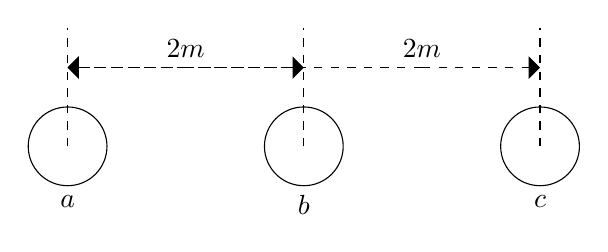
\begin{tikzpicture}
\draw (0,0) circle (.5); \draw (0,-.5) node[below] {$a$}; \draw[dashed] (0,0) -- (0, 1.5);
\draw (3,0) circle (.5); \draw (3,-.5) node[below] {$b$}; \draw[dashed] (3,0) -- (3, 1.5);
\draw (6,0) circle (.5); \draw (6,-.5) node[below] {$c$}; \draw[dashed] (6,0) -- (6, 1.5);

\draw[dashed, -triangle 90] (1.5,1) -- (0,1); \draw[dashed, -triangle 90] (1.5,1) -- (3,1);\draw (1.5,1) node[above] {$2m$};

\draw[dashed, -triangle 90] (4.5,1) -- (0,1); \draw[dashed, -triangle 90] (4.5,1) -- (6,1);\draw (4.5,1) node[above] {$2m$};
\end{tikzpicture}
\end{center}
\caption{Sơ đồ minh họa cho bài tập \ref{Ex-5}} \label{Fig:bai-tap-5}
\end{figure}
	\subparagraph{Bài giải bài tập \ref{Ex-5}}
	\begin{itemize}
		\item Ta có: bán kính dây dẫn $r_a = r_b = r_c = r = \dfrac{2}{2} = 1 \unit{cm} = 0.01 \unit{m}$.
		\item Xác định $D_m$ và $D_s$:
			\begin{align*}
				D_m & =\sqrt[3]{D_{ab} D_{bc} D_{ac}} = \sqrt[3]{2 \times 2 \times 4} = 2.520 \unit{m}\\
				D_s & = \sqrt[3]{r_a r_b r_c} = \sqrt[3]{0.01 \times 0.01 \times 0.01 }= 0.01 \unit{m}
			\end{align*}
		\item Điện dung trên mỗi $km$ chiều dài:
			\begin{align*}
				C_0 =\dfrac{1}{18 \times 10^6 \times  \ln{\dfrac{D_m}{D_s}}} = \dfrac{1}{18 \times 10^{6} \times  \ln{\dfrac{2.520}{0.01}}} = 1 \times 10^{-8} \unitp{F/km} 
			\end{align*}
			
		\item Điện dung trên $100 \unit{km}$ đường dây: $C = C_0 l = 10^{-8} \times 100 = 10^{-6} \unitp{F}$
	\end{itemize}
	\begin{comment}
	\item \label{Ex-6} Một đường dây ba pha lộ kép có hoán vị được cho trên hình \ref{Fig:bai-tap-6}. Bán kính mỗi dây là $1.25 \unit{cm}$. Tính điện cảm trên mỗi $km$ đường dây và điện dung trên mỗi $km$ so với trung tính của mỗi pha.
	\begin{figure}[!h]
\begin{center}
\begin{tikzpicture}
\draw (0,0) circle (.5); \draw (-.5, 0) node[left]{$a$};
\draw (-2,-2) circle (.5); \draw (-2.5, -2) node[left]{$b$};
\draw (0,-4) circle (.5); \draw (-.5, -4) node[left]{$c$};
\draw (4,0) circle (.5); \draw (3.5, 0) node[left]{$c^\prime$};
\draw (6,-2) circle (.5);  \draw (5.5, -2) node[left]{$b^\prime$};
\draw (4,-4) circle (.5); \draw (3.5, -4) node[left]{$a^\prime$};
\draw[dashed] (0,0) -- (0,1.5);
\draw[dashed] (4,0) -- (4,1.5);
\draw[dashed] (-2,-2) -- (-2,-.5);
\draw[dashed] (6,-2) -- (6,-.5);
\draw[dashed] (4,0) -- (8,0);
\draw[dashed] (6,-2) -- (8,-2);
\draw[dashed] (4,-4) -- (8,-4);

\draw[dashed, -triangle 90] (2,1) -- (0,1);
\draw[dashed, -triangle 90] (2,1) -- (4,1); \draw (2,1) node[above] {$7.5m$};

\draw[dashed, -triangle 90] (4,-1) -- (-2,-1);
\draw[dashed, -triangle 90] (4,-1) -- (6,-1); \draw (2,-1) node[above] {$9m$};

\draw[dashed, -triangle 90] (7.5,-1) -- (7.5,0);
\draw[dashed, -triangle 90] (7.5,-1) -- (7.5,-2); \draw (7.5,-1) node[right] {$4m$};

\draw[dashed, -triangle 90] (7.5,-3) -- (7.5,-2);
\draw[dashed, -triangle 90] (7.5,-3) -- (7.5,-4); \draw (7.5,-3) node[right] {$4m$};
\end{tikzpicture}
\end{center}
\caption{Sơ đồ minh họa cho bài tập \ref{Ex-6}} \label{Fig:bai-tap-6}
\end{figure}
\subparagraph{Bài giải bài tập \ref{Ex-6}}
\begin{itemize}
	\item Ta có: bán kính dây dẫn $r = \dfrac{1.25}{2} = 0.625 \unit{cm} = 6.25 \times 10^{-3} \unit{m}$.
	\item  Suy ra: $r^\prime = r e^{-0.25} = 4.868 \times 10^{-3} \unit{m}$.
	\item Ta có:
		\begin{align*}
			D_{a b^\prime} & = \sqrt{\pfm{7.5 + \dfrac{9 - 7.5}{2}}^2 + 4^2} = 9.169 \unit{m}\\
			D_{a^\prime b^\prime} & = \sqrt{\pfm{\dfrac{9 - 7.5}{2}}^2 + 4^2} = 4.070 \unit{m}
		\end{align*}
	\item Xác định $D_m$ và $D_s$:
		\begin{itemize}
			\item Xác định $D_{AB}, D_{BC}, D_{AC}$:
			\begin{align*}
				D_{AB} & = \pfm{D_{ab} D_{ab^\prime} D_{a^\prime b} D_{a^\prime b^\prime}}^{\frac{1}{4}} = \pfm{4.070 \times 9.169 \times 9.169 \times 4.070}^{\frac{1}{4}} = 6.109 \unit{m}\\
				D_{BC} & = \pfm{D_{bc} D_{bc^\prime} D_{b^\prime c} D_{b^\prime c^\prime}}^{\frac{1}{4}} = \pfm{4.070 \times 9.169 \times 9.169 \times 4.070}^{\frac{1}{4}} = 6.109 \unit{m}\\
				D_{AC} & = \pfm{D_{ac} D_{ac^\prime} D_{a^\prime c} D_{a^\prime c^\prime}}^{\frac{1}{4}} = \pfm{8 \times 7.5 \times 7.5 \times 8}^{\frac{1}{4}} = 2.783 \unit{m}
			\end{align*}
			
			\item Suy ra: $D_m = \pfm{D_{AB} D_{BC}D_{AC}}^\frac{1}{3} = \pfm{\sqrt[4]{8} \times \sqrt[4]{8} \times \sqrt[4]{20}} ^\frac{1}{3} = 1.815 \unit{m}$.	
			\item Xác định $D_{sA}, D_{sB}, D_{sC}$:
			\begin{align*}
				D_{sA} & = \sqrt{r^\prime D_{a a^\prime}} = \sqrt{7.88 \times 10^{-3} \times 3} = 0.153 \unit{m}\\
				D_{sB} & = \sqrt{r^\prime D_{b b^\prime}} = \sqrt{7.88 \times 10^{-3} \times 3} = 0.153 \unit{m}\\
				D_{sC} & = \sqrt{r^\prime D_{c c^\prime}} = \sqrt{7.88 \times 10^{-3} \times 3} = 0.153 \unit{m}
			\end{align*}
			\item Suy ra: $D_s = \pfm{D_{sA} D_{sB}D_{sC}}^\frac{1}{3} = \pfm{0.153 \times 0.153 \times 0.153} ^\frac{1}{3} = 0.153 \unit{m}$.
		\end{itemize}
	\item Điện cảm trên mỗi $km$ của mỗi pha trên đường dây mạch kép:
	\begin{align*}
		L_0 = 2 \times 10^{-4} \times \ln{\dfrac{D_m}{D_s}} = 2 \times 10^{-4} \times \ln{\dfrac{1.815}{0.153}} = 4.947 \times 10^{-4} \unitp{H/km}
	\end{align*}
	
	\item Điện kháng trên mỗi $km$ của mỗi pha trên đường dây mạch kép:
		\begin{align*}
			x_0 = 2 \pi f L_0 = 2 \pi \times 50 \times 4.947 \times 10^{-4} = 0.155 \unitp{\Omega /km}
		\end{align*}
\end{itemize}
\end{comment}
\end{enumerate} 		% Các thông số của đường dây truyền tải trên không
\newpage
\section{Tính toán các tham số của đường dây truyền tải}
\subsection{Đường dây truyền tải}
	Với đường dây truyền tải, ta cần khảo sát các thông số: \emph{điện áp}, \emph{dòng điện}, \emph{công suất} và \emph{hệ số công suất} ở \emph{đầu gửi} và \emph{đầu nhận}.\\

	Việc\emph{ lựa chọn đường dây truyền} tải theo yêu cầu: \emph{tổn thất công suất nhỏ nhất}, \emph{hiệu quả cao trong vận hành} và \emph{độ sụt áp trong giới hạn cho phép}.\\
	
	\emph{Phân loại đường dây truyền tải:}
		\begin{itemize}
			\item \emph{Đường dây ngắn:} chiều dài $l <80\unit{km}$.
			
			\item \emph{Đường dây trung bình:} chiều dài $80 \unit{km} \leq l \leq 240 \unit{km}$.
			
			\item \emph{Đường dây dài:} chiều dài $l > 240 \unit{km}$.
		\end{itemize}
		
	\emph{Thông số đường dây:}
		\begin{itemize}
			\item \emph{Tổng trở:} $\overline{Z} = \pfm{r_0+jx_0}l = \pfm{r_0+j\omega L_0}l$.
			\item \emph{Tổng dẫn:} $\overline{Y} = \pfm{g_0+jb_0}l \approx jb_0l =  j\omega C_0 l$.
		\end{itemize}
		
	Gọi $V_S$ và $V_R$ lần lượt là \emph{điện áp pha} đầu gửi và \emph{điện áp pha} đầu nhận.
	\begin{itemize}
		\item Phần trăm sụt áp: $\Delta U \%= \dfrac{V_S - V_R}{V_R} \times 100 \%$

		\item Các công thức tính công suất:
			\begin{align*}
				P & = \sqrt{3}U_{L}I_{L}\cos \varphi = 3U_{P}I_{P}\cos \varphi; &  Q & = \sqrt{3}U_{L}I_{L}\sin \varphi = 3U_{P}I_{P}\sin \varphi;\\
			S & = \sqrt{3}U_{L}I_{L} = 3 U_{P} I_{P}; & \overline{S} & = \sqrt{3}\overline{U}_{L}\overline{I}_{L}^{\ast} = 3\overline{U}_{P}\overline{I}_{P}^{\ast} = P + jQ\\
			P  & = S\cos \varphi; \quad Q  = S\sin \varphi =  P\tan\varphi;  & S & = \sqrt{P^2 + Q^2}
			\end{align*}					
		
		\item Tổn hao công suất trên đường dây truyền tải: $\Delta P = P_S - P_R$.
		
		\item Hiệu suất của đường dây: $\eta = \dfrac{P_R}{P_S} \times 100\%$
		
		\item Hệ số công suất: $\cos \varphi = \cos \pfm{\varphi_{V} - \varphi_{I}}$.
	\end{itemize}
	
	\emph{Mô hình hóa của đường dây truyền tải:}
		\begin{itemize}		
			\item Mô hình hóa: hình \ref{Fig:mo-hinh-hoa-duong-day}.
			\begin{figure}[!h]
				\begin{center}
					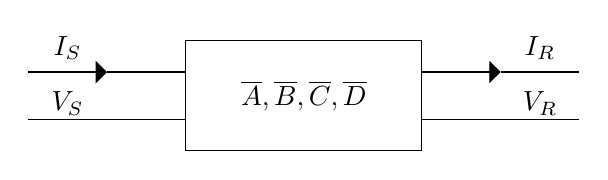
\begin{tikzpicture}
					\draw[-triangle 90] (0,0) -- (1,0);
					\draw (1,0) -- (2,0);
					\draw (2,.4) rectangle (5,-1);
					\draw[-triangle 90] (5,0) -- (6,0);
					\draw (6,0) -- (7,0);
				
					\draw (0,-.6) -- (2,-.6);
					\draw (5,-.6) -- (7,-.6);
					\draw (0.5,0.3) node{$I_S$} ;
					\draw (0.5,-0.4) node{$V_S$} ;
				
					\draw (6.5,0.3) node{$I_R$} ;
					\draw (6.5,-0.4) node{$V_R$} ;
				
					\draw (3.5,-0.3) node{$\overline{A}, \overline{B}, \overline{C}, \overline{D}$};	
				\end{tikzpicture}
			\end{center}
			\caption{Mô hình hóa của đường dây truyền tải} \label{Fig:mo-hinh-hoa-duong-day}
		\end{figure}
		
		\item Phương trình quan hệ dòng điện và điện áp giữa đầu gửi với đầu nhận:
			\begin{align*}
				\left[{\begin{array}{c}
				\overline{V}_S\\
				\overline{I}_S
				\end{array}
				}\right]
				= 
				\left[{\begin{array}{cc}
				\overline{A} & \overline{B}\\
				\overline{C} & \overline{D}
				\end{array}
				}\right]				
				\left[{\begin{array}{c}
				\overline{V}_R\\
				\overline{I}_R
				\end{array}
				}\right]
				\Longleftrightarrow
				 \left\{{\begin{array}{c}
				 \overline{V}_S = \overline{A}.\overline{V}_R + \overline{B}.\overline{I}_R\\
				 \overline{I}_S = \overline{C}.\overline{V}_R + \overline{D}.\overline{I}_R
				 \end{array}
				}\right.
			\end{align*}
			
		\item Với các thông số $\overline{A}, \overline{B}, \overline{C}, \overline{D}$ được xác  định tùy theo \emph{loại đường dây} (đường dây ngắn, đường dây trung bình, đường dây dài) và  \emph{mô hình hóa} của đường dây (mạch $T$ chuẩn, mạch $\Pi$ chuẩn).
	\end{itemize}

\subsection{Công thức tổng quát của mô hình đường dây truyền tải}
	\begin{itemize}
		
		\item Sử dụng công thức tổng quát cho kết quả chính xác hơn so với các công thức gần đúng (các công thức của đường dây trung bình).
		
		\item Công thức tổng quát khai triển \emph{3 số hạng đầu} trong khai triển \emph{Maclaurin}:
			\begin{align*}						
				\overline{A}  = \overline{D} = 1 + \dfrac{\overline{Y}.\overline{Z}}{2} + \dfrac{\overline{Y}^2.\overline{Z}^2}{24}; \quad \overline{B}  = \overline{Z}\pfm{1 + \dfrac{\overline{Y}.\overline{Z}}{6} + \dfrac{\overline{Y}^2.\overline{Z}^2}{120}}; \quad
				 \overline{C} = \overline{Y} \pfm{1 + \dfrac{\overline{Y}.\overline{Z}}{6} + \dfrac{\overline{Y}^2.\overline{Z}^2}{120}}	
			\end{align*}
		\end{itemize}
\subsection{Đường dây truyền tải ngắn}
	\begin{itemize}
		\item Chiều dài đường dây: $l < 80 \unit{km}$.
		
		\item Giá trị của thông số $\overline{A}, \overline{B}, \overline{C}, \overline{D}$ trong mạch tương đương \emph{tổng trở nối tiếp}:
		\begin{align*}
			\overline{A} = \overline{D} = 1; \qquad \overline{B} = \overline{Z}; \qquad \overline{C} = 0
		\end{align*}
		
		\item Sơ đồ tương đương cho đường dây ngắn: hình \ref{Fig:mach-tuong-duong-duong-day-ngan}.
			\begin{figure}[!h]
			\begin{center}				
				\begin{circuitikz}
					\draw (0,0) to [european resistor, *-, l_ = $R$] (3,0) to [L, l_ = $jX$] (6,0) to [short, i_ = $ $, l_ = \text{$\dot{I} = \dot{I}_{S} = \dot{I}_{R}$}] (9,0) to [european resistor, l_ = $Load$] (9,-3) to [short, -*] (0,-3);
					\draw (.5,0) to [open, l_= \text{$\dot{V}_S$}] (.5,-3);
					\draw (6,0) to [open, l_= \text{$\dot{V}_R$}] (6,-3);
					\draw[<->] (0.5,-.2) -- (.5,-2.8);% node[below] {$\dot{V}_S$};	
					\draw[<->] (6,-.2) -- (6,-2.8);%node[below] {$\dot{V}_R$};					
				\end{circuitikz}
			\end{center}
			\caption{Mạch tương đương cho đường dây ngắn (pha với trung tính)} \label{Fig:mach-tuong-duong-duong-day-ngan}
			\end{figure}
	\end{itemize}
	
\subsection{Đường dây truyền tải trung bình}
	\begin{itemize}
		\item Chiều dài đường dây: $80 \unit{km} \leq l \leq  240 \unit{km}$.
		\item Giá trị của thông số $\overline{A}, \overline{B}, \overline{C}, \overline{D}$
			\begin{itemize}	
				\item Mạch tương đương $T$ \emph{chuẩn}:
					\begin{align*}
						\overline{A} = \overline{D} = 1 + \dfrac{\overline{Y}. \overline{Z}}{2}; \qquad \overline{B} = \overline{Z}\pfm{1 + \dfrac{\overline{Y} . \overline{Z}}{4}}; \qquad \overline{C} = \overline{Y}
					\end{align*}
		
			\item Mạch tương đương $\Pi$ \emph{chuẩn}:
				\begin{align*}
					\overline{A} = \overline{D} = 1 + \dfrac{\overline{Y}. \overline{Z}}{2}; \qquad \overline{B} = \overline{Z}; \qquad \overline{C} = \overline{Y}\pfm{1 + \dfrac{\overline{Y} . \overline{Z}}{4}}
				\end{align*}
			\item Sơ đồ tương đương cho đường dây trung bình:
				\begin{itemize}			
				\item Sơ đồ tương đường hình $T$ chuẩn: hình \ref{Fig:mach-tuong-duong-duong-day-trung-binh-T}.
			\begin{figure}[!h]
			\begin{center}				
				\begin{circuitikz}
					\draw (-1,0) to [short, *-] (0,0) to [european resistor, l_ = $\frac{1}{2}R$] (2,0) to [L, l_ = $j\frac{1}{2}X$] (4,0) to [short] (6,0) to [european resistor, l_ = $\frac{1}{2}R$] (8,0) to [L, l_ = $j\frac{1}{2}X$] (10, 0) to [short] (12, 0) to [european resistor, l_ = $Load$] (12,-4) to [short, -*] (-1,-4);
					\draw (5,0) to [C, l_=\text{$\dot{Y} = jB$}] (5,-4);
					\draw (5,0) to [short, i_ = $\dot{I}_R$] (6.4,0);
					\draw (-1,0) to [short, i_ = $\dot{I}_S$] (0.3,0);
					\draw (5,-2.5) to [short, i_ = $\dot{I}_C$] (5,-4);
					\draw (0,0) to [open, l_= \text{$\dot{V}_S$}] (0,-4);
					\draw (10,0) to [open, l_= \text{$\dot{V}_R$}] (10,-4);
					\draw[<->] (0,-.2) -- (0,-3.8);% node[below] {$\dot{V}_S$};	
					\draw[<->] (10,-.2) -- (10,-3.8);% node[below] {$\dot{V}_R$};					
				\end{circuitikz}
			\end{center}
			\caption{Mạch tương đương hình $T$ chuẩn cho đường dây trung bình} \label{Fig:mach-tuong-duong-duong-day-trung-binh-T}
			\end{figure}
			
			\item Sơ đồ tương đường hình $\Pi$ chuẩn: hình \ref{Fig:mach-tuong-duong-duong-day-trung-binh-Pi}.
			\begin{figure}[!h]
			\begin{center}				
				\begin{circuitikz}
					\draw(-3,0) to [short,*-] (0,0) to [european resistor, l_ = $R$] (3,0) to [L, l_ = $jX$] (6,0) to [short] (8,0) to [short, i_ = $ $, l_ = \text{$\dot{I}_{R}$}] (10,0) to [european resistor, l_ = $Load$] (10,-4) to [short, -*] (-3,-4);
					\draw (6,0) to [C, l_=\text{$\frac{\dot{Y}}{2} = j\frac{B}{2}$}] (6,-4);
					\draw (6,-2.5) to [short, i_ = $\dot{I}_C$] (6,-4);
					\draw (0,0) to [C, l_=\text{$\frac{\dot{Y}}{2} = j\frac{B}{2}$}] (0,-4);
					\draw (-2.5,0) to [open, l_= \text{$\dot{V}_S$}] (-2.5,-4);
					\draw (8,0) to [open, l_= \text{$\dot{V}_R$}] (8,-4);
					\draw[<->] (-2.5,-.2) -- (-2.5,-3.8);% node[below] {$\dot{V}_S$};	
					\draw[<->] (8,-.2) -- (8,-3.8);%node[below] {$\dot{V}_R$};					
				\end{circuitikz}
			\end{center}
			\caption{Mạch tương đương hình $\Pi$ chuẩn cho đường dây trung bình} \label{Fig:mach-tuong-duong-duong-day-trung-binh-Pi}
			\end{figure}
			\end{itemize}
		\end{itemize}
	\end{itemize}
	
\subsection{Đường dây truyền tải dài}
	\begin{itemize}
		\item Chiều dài đường dây: $l >  240 \unit{km}$.
		
		\item Giá trị của thông số $\overline{A}, \overline{B}, \overline{C}, \overline{D}$ trong mạch tương đương  \emph{thông số rãi}:
		\begin{align*}
			\overline{A} = \overline{D} = \cosh \theta; \qquad \overline{B} = \overline{Z}_C \sinh \theta; \qquad \overline{C} = \dfrac{\sinh\theta}{\overline{Z}_C}
		\end{align*}
		với $\theta = l\sqrt{\overline{z}.\overline{y}}$ và $\overline{Z}_C = \sqrt{\dfrac{\overline{z}}{\overline{y}}}$.
		\item Một số \emph{công thức liên quan đến số phức} cần cho mô hình tính toán đường dây dài:
			\begin{itemize}		
		 		\item[$\ast$] Căn bậc hai của số phức: $w = \pfm{r\angle \varphi}^\frac{1}{2} = \sqrt{r} \angle \dfrac{\varphi}{2}$
		 		\item[$\ast$] Hàm lượng giác \emph{hyperbolic} với số phức (khi tính toán chuyển sang chế độ \emph{radian}): 
		 			\begin{align*}
		 				\sinh \pfm{a+jb} & = \sinh a \cos b + j\cosh a \sin b\\
		 				\cosh \pfm{a+jb} & = \cosh a \cos b + j\sinh a \sin b
		 			\end{align*}
				\item[$\ast$] Hàm lượng giác của hàm \emph{hyperbolic}:
			\begin{align*}
				\sinh \theta = \dfrac{e^\theta- e^{-\theta} }{2}; \qquad \cosh  \theta = \dfrac{e^\theta + e^{-\theta} }{2}
			\end{align*}
		\end{itemize}
		\item Sơ đồ tương đương cho đường dây dài: hình \ref{Fig:mach-tuong-duong-duong-day-dai}.
			\begin{figure}[!h]
			\begin{center}				
				\begin{circuitikz}
					\draw (0,0) to [short, *-, i_ = $I_S$] (1, 0) to [european resistor, l_ = $r$] (3,0) to [L, l_ = $jx$] (5,0) to [short] (6.5,0) to [european resistor, l_ = $r$] (8.5,0) to [L, l_ = $jx$] (10.5,0) to [short] (12,0) to [european resistor, l_ = $r$] (14,0) to [L, l_ = $jx$] (16,0) to [short, i_ = $\dot{I}_S$] (18,0) to [european resistor, l_=$Load$] (18,-4) to [short, -*] (0,-4);
					\draw (5.75, 0) to [short] (5.75,-1) to [short] (6.75,-1) to [C, l_ = $jb$] (6.75,-3) to [short] (4.75,-3) to [european resistor, l_=$g$] (4.75,-1) to [short] (5.75,-1);
					\draw (5.75,-3) to [short] (5.75,-4);
					
					\draw (11.25, 0) to [short] (11.25,-1) to [short] (12.25,-1) to [C, l_ = $jb$] (12.25,-3) to [short] (10.25,-3) to [european resistor, l_=$g$] (10.25,-1) to [short] (11.25,-1);
					\draw (11.25,-3) to [short] (11.25,-4);
					
					\draw (1,0) to [open, l_= \text{$\dot{V}_S$}] (1,-4);
					\draw (16,0) to [open, l_= \text{$\dot{V}_R$}] (16,-4);
					\draw[<->] (1,-.2) -- (1,-3.8);% node[below] {$\dot{V}_S$};	
					\draw[<->] (16,-.2) -- (16,-3.8);%node[below] {$\dot{V}_R$};					
				\end{circuitikz}
			\end{center}
			\caption{Các thông số rãi của đường dây truyền tải dài} \label{Fig:mach-tuong-duong-duong-day-dai}
			\end{figure}
	\end{itemize}
\subsection{Bài tập tính toán các tham số của đường dây truyền tải}
	\begin{enumerate}
		\item \label{Ex-tham-so-duong-day:bt1} Một đường dây 3 pha, $11 \unit{kV}$, dài $10 \unit{km}$ chuyển cho đầu nhận tải $5000 \unit{kW}$, $\cos \varphi_R = 0.8$ (trễ). Điện trở mỗi pha trên một $km$ là $0.1 \unit{\Omega}$ và cảm kháng mỗi pha trên một $km$ là $0.2 \unit{\Omega}$. Tính:
			\begin{enumerate}[a.]
				\item Vẽ sơ đồ thay thế cho mô hình đường dây ngắn.
				\item Các thông số $\overline{A}, \overline{B}, \overline{C}, \overline{D}$ của đường dây.
				\item Điện áp và dòng điện đầu gửi.
				\item Hệ số công suất đầu gửi.
				\item Góc lệnh pha giữa điện áp đầu gửi và đầu nhận.
				\item Độ sụt áp.
				\item Công suất tác dụng, phản kháng và biểu kiến ở đầu gửi.
				\item Tổn thất công suất trên đường dây.
				\item Hiệu suất truyền tải.
				\item Vẽ giản đồ vector.
				\item[$\ast$] \emph{Lưu ý:} Làm tròn kết quả \emph{2 chữ số} sau dấu phẩy.
			\end{enumerate}
			
		\subparagraph{Bài giải bài tập \ref{Ex-tham-so-duong-day:bt1}}
			\begin{enumerate}[\it a.]
				\item[$\bullet$] Ta có: $\overline{Z} = \pfm{r_0 + j x_0}l = \pfm{0.1 +j 0.2}\times 10 = 1 + j 2 = 2.24 \angle 63.43^0 \unitp{\Omega}$.
					
				\item[$\bullet$] Chọn $\overline{V}_R = \dfrac{11}{\sqrt{3}} \angle 0^0 = 6.35 \angle 0^0 \unitp{kV} $
				
				\item[$\bullet$] Suy ra: $I_R = \dfrac{P_R}{\sqrt{3}V_R \cos \varphi} = \dfrac{5\times 10^3}{\sqrt{3} \times 11 \times 0.8} = 0.33 \times 10^3 \unit{A} = 0.33\unitp{kA}$.
				
				\item[$\bullet$] Có $\cos \varphi_R = 0.8$ (trễ) $ \Longrightarrow \varphi_R  = +36.87^0$.				
				\item[$\bullet$] Có $\varphi_R = \varphi_{V_R} - \varphi_{I_R} \Longrightarrow \varphi_{I_R} = \varphi_{V_R} - \varphi_R = 0^0 - 36.87^0 = -36.87^0$.
				\item[$\bullet$] Nên: $\overline{I}_R = 0.33 \angle -36.87^0 \unitp{kA}$ .

				\item \emph{Sơ đồ tương đương cho đường dây ngắn:} hình \ref{Fig:mach-tuong-duong-duong-day-ngan-bt1}.
			\begin{figure}[!h]
			\begin{center}				
				\begin{circuitikz}
					\draw (0,0) to [european resistor, *-, l_ = $1\unit{\Omega}$] (3,0) to [L, l_ = $j2 \unit{\Omega}$] (6,0) to [short, i_ = $ $, l_ = \text{$\dot{I} = \dot{I}_{S} = \dot{I}_{R}$}] (9,0) to [european resistor, l_ = $Load$] (9,-3) to [short, -*] (0,-3);
					\draw (.5,0) to [open, l_= \text{$\dot{V}_S$}] (.5,-3);
					\draw (6,0) to [open, l_= \text{$\dot{V}_R$}] (6,-3);
					\draw[<->] (0.5,-.2) -- (.5,-2.8);% node[below] {$\dot{V}_S$};	
					\draw[<->] (6,-.2) -- (6,-2.8);%node[below] {$\dot{V}_R$};					
				\end{circuitikz}
			\end{center}
			\caption{Mạch tương đương cho đường dây ngắn trong bài tập \ref{Ex-tham-so-duong-day:bt1}} \label{Fig:mach-tuong-duong-duong-day-ngan-bt1}
			\end{figure}				
				\newpage
				\item \emph{Thông số $\overline{A}, \overline{B}, \overline{C}, \overline{D}$ cho mô hình đường dây ngắn}				
					\begin{align*}
						\overline{A} 	= \overline{D}  = 1; \qquad \overline{B} = \overline{Z} = 2.24 \angle 63.43^0 \unitp{\Omega}; \qquad \overline{C} = 0
					\end{align*}
				
				\item \emph{Xác định điện áp đầu gửi $\overline{V}_S$ và dòng điện đầu gửi $\overline{I}_S$}
					\begin{itemize}
						\item Ta có: 
							\begin{align*}
								\left[{\begin{array}{c}
								\overline{V}_S\\
								\overline{I}_S
								\end{array}
								}\right]
								= 
								\left[{\begin{array}{cc}
								\overline{A} & \overline{B}\\
								\overline{C} & \overline{D}
								\end{array}
								}\right]				
							\left[{\begin{array}{c}
							\overline{V}_R\\
							\overline{I}_R
							\end{array}
							}\right]
							= \left[{\begin{array}{cc}
								1 & 2.24 \angle 63.43^0\\
								0 & 1
								\end{array}
								}\right]				
							\left[{\begin{array}{c}
							6.35 \angle 0^0\\
							0.33 \angle -36.87^0
							\end{array}
							}\right]
						\end{align*}
						
						\item Điện áp đầu gửi:
							\begin{align*}
								\overline{V}_S  = \overline{A}. \overline{V}_R + \overline{B}.\overline{I}_R = 1 \times 6.35 \angle 0^0 + 2.24 \angle 63.43^0 \times 0.33 \angle -36.87^0 = 7.02 \angle 2.70^0 \unitp{kV}
								\end{align*}
								
						\item Điện áp dây đầu gửi: $V_{LS}  = \sqrt{3} V_R = \sqrt{3} \times 7.02 = 12.16 \unitp{kV}$.
						\item Dòng điện đầu gửi:
							\begin{align*}								
								\overline{I}_S  = \overline{C}. \overline{V}_R + \overline{D}.\overline{I}_R = 0 \times 6.35 \angle 0^0 + 1 \times 0.33 \angle -36.87^0 = 0.33 \angle -36.87^0 \unitp{kA}
							\end{align*}
					\end{itemize}

					\item \emph{Xác định hệ số công suất đầu gửi $\cos \varphi_S$}
						\begin{align*}
							\cos \varphi_S  = \cos \pfm{\varphi_{V_s} - \varphi_{I_{s}}}= \cos \left[{2.70^0 - \pfm{-36.87^0}} \right] = \cos 39.57^0 = 0.77
						\end{align*}
				
				\item \emph{Xác định góc lệch pha giữa điện áp đầu gửi và đầu nhận $\Delta \varphi_V$}
					\begin{align*}
						\Delta \varphi_V = \varphi_{V_S} - \varphi_{V_R} = 2.70^0 - 0^0 = 2.70^0
					\end{align*}
					
				\item \emph{Xác định độ sụt áp $\Delta U$}
					\begin{align*}
						\Delta U \%= \dfrac{V_S - V_R}{V_R} \times 100 \% = \dfrac{7.02 - 6.35}{6.35} \times 100 \% = 10.55\%
					\end{align*}
					
				\item \emph{Xác định công suất tác dụng, phản kháng và biểu kiến ở đầu gửi $P_S, Q_S, S_S$}
					\begin{align*}
						& \overline{S}_S  = 3 \overline{V}_S.\overline{I}_S^{\ast} = 3 \times 7.02 \angle 2.70^0 \times 0.33 \angle +36.87^0 = 5.36 + j4.43 \unitp{MVA}\\
						\Longrightarrow & P_S  = 5.36 \unit{MW}; \qquad Q_S = 4.43 \unit{MVAr}
					\end{align*}
				\item \emph{Xác định tổn thất công suất $\Delta P$}
					\begin{align*}
						\Delta P = P_S - P_R = 5.36 - 5 = 0.36 \unitp{MW}
					\end{align*}
				
				\item \emph{Xác định hiệu suất $\eta$}
						\begin{align*}
							\eta = \dfrac{P_R}{P_S} \times 100 \% = \dfrac{5}{5.36} \times 100\% = 93.28\%
						\end{align*}
					
				\item \emph{Vẽ giản đồ vector:} hình \ref{Fig:gian-do-vector-bt1}.
					\begin{figure}[!h]
						\begin{center}
							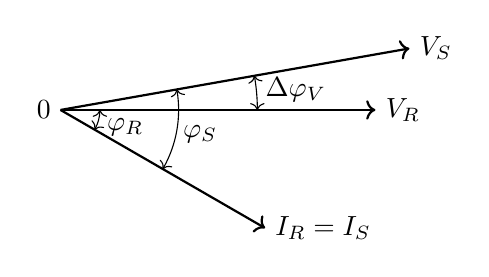
\begin{tikzpicture}
								\coordinate (origo) at (0,0);
								\coordinate (pivot) at (1,5);
    
    							\draw (0,0) node[left] {$0$};
    							\draw[thick,->] (origo) -- ++(4,0) node (VR) [right] {$V_R$};

								\draw[thick,->] (origo) -- ++(330:3) coordinate (IR) node[right] {$I_R =  I_S$};
    
							    \draw[thick,->] (origo) -- ++(370:4.5) coordinate (VS) node[right] {$V_S$};

								\pic [draw, <->, "$\varphi_R$", angle eccentricity=1.7] {angle = IR--origo--VR};
    
								\pic [draw, <->, "$\varphi_S$", angle eccentricity=1.2, angle radius=1.5cm] {angle = IR--origo--VS};
    
							    \pic [draw, <->, "$\Delta \varphi_V$", angle eccentricity=1.2, angle radius=2.5cm] {angle = VR--origo--VS};
							\end{tikzpicture} \hspace{1cm}							
							 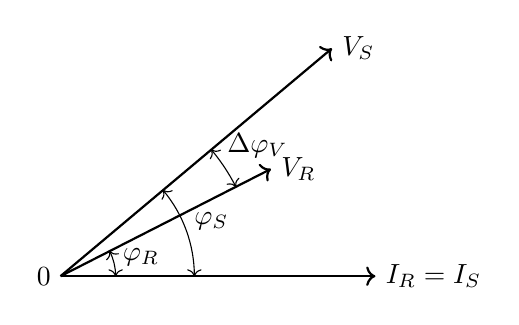
\begin{tikzpicture}
    							\coordinate (origo) at (0,0);
   								\coordinate (pivot) at (1,5);
    
    							\draw (0,0) node[left] {$0$};
							    \draw[thick,->] (origo) -- ++(4,0) node (IR) [right] {$I_R = I_S$};

							    \draw[thick,->] (origo) -- ++(387:3) coordinate (VR) node[right] {$V_R$};
    
							    \draw[thick,->] (origo) -- ++(400:4.5) coordinate (VS) node[right] {$V_S$};

							    \pic [draw, <->, "$\varphi_R$", angle eccentricity=1.5, angle radius=.7cm] {angle = IR--origo--VR};
    
							    \pic [draw, <->, "$\varphi_S$", angle eccentricity=1.2, angle radius=1.7cm] {angle = IR--origo--VS};
    
								\pic [draw, <->, "$\Delta \varphi_V$", angle eccentricity=1.2, angle radius=2.5cm] {angle = VR--origo--VS};
						  \end{tikzpicture}
						\end{center}
						\caption{Giản đồ vector cho bài tập \ref{Ex-tham-so-duong-day:bt1}} \label{Fig:gian-do-vector-bt1}
					\end{figure}
			\end{enumerate}
		
		\item \label{Ex-tham-so-duong-day:bt2} Một đường dây 3 pha, $110 \unit{kV}$, $f=50Hz$, dài $150 \unit{km}$ chuyển cho đầu nhận tải $40000 \unit{kW}$, $\cos \varphi_R = 0.8$ (trễ). Điện trở mỗi pha trên một $km$ là $0.15 \unit{\Omega}$,  dung dẫn mỗi pha trên một $km$ là $10 \times 10^{-6} \unit{\Omega^{-1}}$ và cảm kháng mỗi pha trên một $km$ là $0.6 \unit{\Omega}$. Thực hiện tính toán trên 3 mô hình: \emph{mô hình $T$ chuẩn},  \emph{mô hình $\Pi$ chuẩn} và \emph{mô hình tổng quát}.
			\begin{enumerate}[a.]
				\item Vẽ sơ đồ thay thế cho mô hình đường dây trung bình cho mạch tương ứng.
				\item Các thông số $\overline{A}, \overline{B}, \overline{C}, \overline{D}$ của đường dây.
				\item Điện áp và dòng điện đầu gửi.
				\item Độ lệch pha giữa điện áp đầu gửi và đầu nhận.
				\item Hệ số công suất đầu gửi.
				\item Công suất tác dụng, phản kháng và biểu kiến ở đầu gửi.
				\item Tổn thất công suất trên đường dây.
				\item Độ sụt áp của đường dây.
				\item Hiệu suất truyền tải.
				\item Vẽ giản đồ vector.
				\item[$\ast$] \emph{Lưu ý:} Làm tròn kết quả \emph{2 chữ số} sau dấu phẩy.
			\end{enumerate}
			
		\subparagraph{Bài giải bài tập \ref{Ex-tham-so-duong-day:bt2}}
			\begin{enumerate}[ \it a.]
				\item[$\bullet$] Ta có:
					\begin{align*}
						\overline{Z} & = \pfm{r_0 + j x_0}l = \pfm{0.15 +j 0.6}\times 150 = 22.5 + j 90 = 92.77 \angle 75.96^0 \unitp{\Omega}\\
						\overline{Y} & = \pfm{g_0 + j b_0}l \approx j b_0 l = j 10 \times 10^{-6}\times 150 = j 1.5 \times 10^{-3} = 1.5 \times 10^{-3} \angle 90^0 \unitp{\Omega^{-1}}
					\end{align*}
				
				\item[$\bullet$] Chọn $\overline{V}_R = \dfrac{110}{\sqrt{3}} \angle 0^0 = 63.51 \angle 0^0 \unitp{kV} $
				\item[$\bullet$] Suy ra: $I_R = \dfrac{P_R}{\sqrt{3}V_R \cos \varphi_R} = \dfrac{40 \times 10^3} {\sqrt{3} \times 110 \times 0.8} = 0.26 \times 10^3 \unit{A} = 0.26\unitp{kA}$.
				
				\item[$\bullet$] Có $\cos \varphi_R = 0.8$ (trễ) $\Longrightarrow \varphi_R  = 36.87^0$.
				\item[$\bullet$] Có $\varphi_R = \varphi_{V_R} - \varphi_{I_R} \Longrightarrow \varphi_{I_R} = \varphi_{V_R} - \varphi_R = 0^0 - 36.87^0 = -36.87^0$.
				\item[$\bullet$] Nên: $\overline{I}_R = 0.26 \angle -36.87^0 \unitp{kA}$ .				
				
				\item[$\star$] \textbf{Mô hình $\mathbf{T}$ chuẩn}
				\item \emph{Sơ đồ tương đường hình $T$ chuẩn:} hình \ref{Fig:mach-tuong-duong-duong-day-trung-binh-T-bt2}.
			\begin{figure}[!h]
			\begin{center}				
				\begin{circuitikz}
					\draw (-1,0) to [short, *-] (0,0) to [european resistor, l_ = $11.25 \unit{\Omega}$] (2,0) to [L, l_ = $j45 \unit{\Omega}$] (4,0) to [short] (6,0) to [european resistor, l_ = $11.25 \unit{\Omega}$] (8,0) to [L, l_ = $j45 \unit{\Omega}$] (10, 0) to [short] (12, 0) to [european resistor, l_ = $Load$] (12,-4) to [short, -*] (-1,-4);
					\draw (5,0) to [C, l_=\text{$j 1.5 \times 10^{-3} \unit{\Omega}^{-1}$}] (5,-4);
					\draw (5,0) to [short, i_ = $\dot{I}_R$] (6.4,0);
					\draw (-1,0) to [short, i_ = $\dot{I}_S$] (0.3,0);
					\draw (5,-2.5) to [short, i_ = $\dot{I}_C$] (5,-4);
					\draw (0,0) to [open, l_= \text{$\dot{V}_S$}] (0,-4);
					\draw (10,0) to [open, l_= \text{$\dot{V}_R$}] (10,-4);
					\draw[<->] (0,-.2) -- (0,-3.8);% node[below] {$\dot{V}_S$};	
					\draw[<->] (10,-.2) -- (10,-3.8);% node[below] {$\dot{V}_R$};					
				\end{circuitikz}
			\end{center}
			\caption{Mạch tương đương hình $T$ cho đường dây trung bình trong bài tập \ref{Ex-tham-so-duong-day:bt2}} \label{Fig:mach-tuong-duong-duong-day-trung-binh-T-bt2}
			\end{figure}
			
				\item \emph{Thông số $\overline{A}, \overline{B}, \overline{C}, \overline{D}$ cho mô hình $T$ chuẩn}				
					\begin{align*}
						\overline{A} 	& = \overline{D}  = 1 + \dfrac{\overline{Y}.\overline{Z}}{2} = 1 + \dfrac{1.5 \times 10^{-3} \angle 90^0 \times 92.77 \angle 75.96^0}{2} = 0.93 \angle 1.04^0\\
						 \overline{B} & = \overline{Z} \pfm{1+\dfrac{\overline{Y}.\overline{Z}}{4}}=92.77 \angle 75.96^0  \pfm{1 + \dfrac{1.5 \times 10^{-3} \angle 90^0 \times 92.77 \angle 75.96^0}{4}} \\ 
						 & \hspace{3.15cm}= 89.64 \angle 76.46^0 \unitp{\Omega}\\
						 \overline{C} & = \overline{Y} = 1.5 \times 10^{-3} \angle 90^0 \unitp{\Omega^{-1}}
					\end{align*}				
				
				\item \emph{Xác định điện áp đầu gửi $\overline{V}_S$ và dòng điện đầu gửi $\overline{I}_S$}
					\begin{itemize}
						\item Ta có: 
							\begin{align*}
								\left[{\begin{array}{c}
								\overline{V}_S\\
								\overline{I}_S
								\end{array}
								}\right]
								= 
								\left[{\begin{array}{cc}
								\overline{A} & \overline{B}\\
								\overline{C} & \overline{D}
								\end{array}
								}\right]				
							\left[{\begin{array}{c}
							\overline{V}_R\\
							\overline{I}_R
							\end{array}
							}\right]
							= \left[{\begin{array}{cc}
								 0.93 \angle 1.04^0 & 89.64 \angle 76.46^0\\
								1.5 \times 10^{-3} \angle 90^0 &  0.93 \angle 1.04^0
								\end{array}
								}\right]				
							\left[{\begin{array}{c}
							63.51 \angle 0^0\\
							0.26 \angle -36.87^0
							\end{array}
							}\right]
						\end{align*}
						
						\item Điện áp đầu gửi:
							\begin{align*}
								\overline{V}_S  & = \overline{A}. \overline{V}_R + \overline{B}.\overline{I}_R  = 0.93 \angle 1.04^0 \times 63.51 \angle 0^0+ 89.64 \angle 76.46^0 \times 0.26 \angle -36.87^0\\
								& \hspace{3cm}= 78.64 \angle 11.68^0 \unitp{kV}
							\end{align*}
						
						\item Điện áp dây đầu gửi: $V_{LS} = \sqrt{3} \times V_S = \sqrt{3} \times 78.64 = 136.21 \unitp{kV}$.						
						
						\item Dòng điện đầu gửi:
							\begin{align*}
								\overline{I}_S & = \overline{C}. \overline{V}_R + \overline{D}.\overline{I}_R = 1.5 \times 10^{-3} \angle 90^0 \times 63.51 \angle 0^0 + 0.93 \angle 1.04^0 \times 0.26 \angle -36.87^0 \\ 
								& \hspace{3cm}= 0.20 \angle -13.28^0 \unitp{kA}
							\end{align*}
					\end{itemize}					
				
				\item \emph{Xác định góc lệch pha giữa điện áp đầu gửi và đầu nhận $\Delta \varphi_V$}
						\begin{align*}
							\Delta \varphi_V = \varphi_{V_S} - \varphi_{V_R} = 11.68^0 - 0^0 = 11.68^0
						\end{align*}
					
				\item \emph{Xác định hệ số công suất đầu gửi $\cos \varphi_S$}
					\begin{align*}
						\cos \varphi_S  = \cos \pfm{\varphi_{V_s} - \varphi_{I_{s}}}= \cos \left[{11.68^0 - \pfm{-13.28^0}} \right] = \cos 24.96^0 = 0.91	
					\end{align*}							
				
				\item \emph{Xác định công suất tác dụng, phản kháng và biểu kiến ở đầu gửi $P_S, Q_S, S_S$}
					\begin{align*}
						&\overline{S}_S  = 3 \overline{V}_S.\overline{I}_S^{\ast} = 3 \times 78.64 \angle 11.68^0 \times 0.20 \angle +13.28^0 = 42.78 + j19.91 \unitp{MVA}\\
						\Longrightarrow & P_S  = 42.78 \unit{MW}; \qquad Q_S = 19.91 \unit{MVAr}
					\end{align*}
					
				\item \emph{Xác định tổn thất công suất $\Delta P$}
					\begin{align*}
						\Delta P = P_S - P_R = 42.78 - 40 = 2.78 \unitp{MW}
					\end{align*}
									
				\item \emph{Xác định độ sụt áp $\Delta U$}
					\begin{align*}
						\Delta U \%= \dfrac{V_S - V_R}{V_R} \times 100 \% = \dfrac{78.64 - 63.51}{63.51} \times 100 \% = 23.82\%
					\end{align*}		
				
				\item \emph{Xác định hiệu suất $\eta$}
						\begin{align*}
							\eta = \dfrac{P_R}{P_S} \times 100 \% = \dfrac{40}{42.78} \times 100\% = 93.50\%
						\end{align*}	
						
				\item \emph{Vẽ giản đồ vector:} hình \ref{Fig:gian-do-vector-bt2}.
					\begin{figure}[!h]
						\begin{center}
							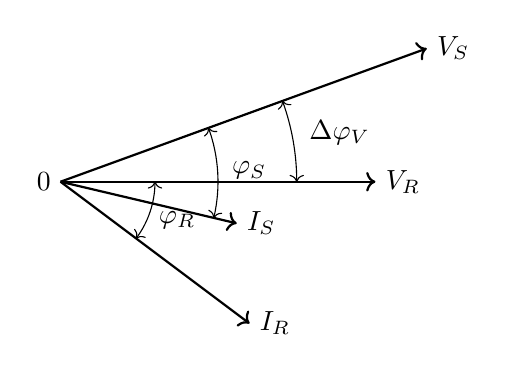
\begin{tikzpicture}
								\coordinate (origo) at (0,0);
								\coordinate (pivot) at (1,5);
    
    							\draw (0,0) node[left] {$0$};
    							\draw[thick,->] (origo) -- ++(4,0) node (VR) [right] {$V_R$};

								\draw[thick,->] (origo) -- ++(323.13:3) coordinate (IR) node[right] {$I_R$};
								
								\draw[thick,->] (origo) -- ++(346.72:2.3) coordinate (IS) node[right] {$I_S$};
    
							    \draw[thick,->] (origo) -- ++(380:4.95) coordinate (VS) node[right] {$V_S$};

								\pic [draw, <->, "$\varphi_R$", angle eccentricity=1.3, angle radius=1.2cm] {angle = IR--origo--VR};
    
								\pic [draw, <->, "$\varphi_S$", angle eccentricity=1.2, angle radius=2cm] {angle = IS--origo--VS};
    
							    \pic [draw, <->, "$\Delta \varphi_V$", angle eccentricity=1.2, angle radius=3cm] {angle = VR--origo--VS};
							\end{tikzpicture} \hspace{1cm}							
							 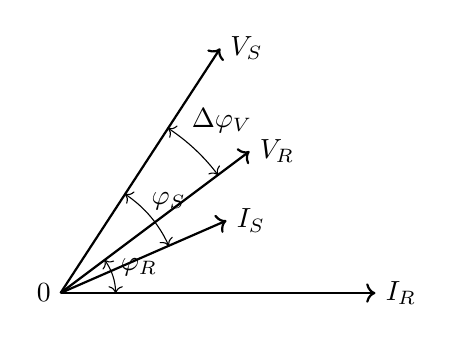
\begin{tikzpicture}
    							\coordinate (origo) at (0,0);
   								\coordinate (pivot) at (1,5);
    
    							\draw (0,0) node[left] {$0$};
							    \draw[thick,->] (origo) -- ++(4,0) node (IR) [right] {$I_R$};

								\draw[thick,->] (origo) -- ++(383.59:2.3) coordinate (IS) node[right] {$I_S$};
								
							    \draw[thick,->] (origo) -- ++(396.87:3) coordinate (VR) node[right] {$V_R$};
    
							    \draw[thick,->] (origo) -- ++(416.87:3.71) coordinate (VS) node[right] {$V_S$};

							    \pic [draw, <->, "$\varphi_R$", angle eccentricity=1.5, angle radius=.7cm] {angle = IR--origo--VR};
    
							    \pic [draw, <->, "$\varphi_S$", angle eccentricity=1.2, angle radius=1.5cm] {angle = IS--origo--VS};
    
								\pic [draw, <->, "$\Delta \varphi_V$", angle eccentricity=1.2, angle radius=2.5cm] {angle = VR--origo--VS};
						  \end{tikzpicture}
						\end{center}
						\caption{Giản đồ vector cho bài tập \ref{Ex-tham-so-duong-day:bt2}} \label{Fig:gian-do-vector-bt2}
					\end{figure}
													
			\end{enumerate}
			\begin{enumerate}[\it a.]
				\item[$\star$] \textbf{Mô hình $\mathbf{\Pi}$ chuẩn}
				\item \emph{Sơ đồ tương đường hình $\Pi$ chuẩn:} hình \ref{Fig:mach-tuong-duong-duong-day-trung-binh-Pi-bt2}.
			\begin{figure}[!h]
			\begin{center}				
				\begin{circuitikz}
					\draw(-5,0) to [short,*-] (0,0) to [european resistor, l_ = $22.5 \unit{\Omega}$] (3,0) to [L, l_ = $j90 \unit{\Omega}$] (6,0) to [short] (8,0) to [short, i_ = $ $, l_ = \text{$\dot{I}_{R}$}] (10,0) to [european resistor, l_ = $Load$] (10,-4) to [short, -*] (-5,-4);
					\draw (6,0) to [C, l_=\text{$j0.75 \times 10^{-3} \unit{\Omega}^{-1}$}] (6,-4);
					\draw (6,-2.5) to [short, i_ = $\dot{I}_C$] (6,-4);
					\draw (0,0) to [C, l_=\text{$j0.75 \times 10^{-3} \unit{\Omega}^{-1}$}] (0,-4);
					\draw (-4,0) to [open, l_= \text{$\dot{V}_S$}] (-4,-4);
					\draw (8,0) to [open, l_= \text{$\dot{V}_R$}] (8,-4);
					\draw[<->] (-4,-.2) -- (-4,-3.8);% node[below] {$\dot{V}_S$};	
					\draw[<->] (8,-.2) -- (8,-3.8);%node[below] {$\dot{V}_R$};					
				\end{circuitikz}
			\end{center}
			\caption{Mạch tương đương hình $\Pi$ cho đường dây trung bình trong bài tập \ref{Ex-tham-so-duong-day:bt2}} \label{Fig:mach-tuong-duong-duong-day-trung-binh-Pi-bt2}
			\end{figure}
			
				\item \emph{Thông số $\overline{A}, \overline{B}, \overline{C}, \overline{D}$ cho mô hình $\Pi$ chuẩn}				
					\begin{align*}
						\overline{A} 	& = \overline{D}  = 1 + \dfrac{\overline{Y}.\overline{Z}}{2} = 1 + \dfrac{1.5 \times 10^{-3} \angle 90^0 \times 92.77 \angle 75.96^0}{2} = 0.93 \angle 1.04^0\\
						 \overline{B} & = \overline{Z} =92.77 \angle 75.96^0  \unitp{\Omega} \\ 
						 \overline{C} & = \overline{Y} \pfm{1+\dfrac{\overline{Y}.\overline{Z}}{4}}= 1.5 \times 10^{-3} \angle 90^0  \pfm{1 + \dfrac{1.5 \times 10^{-3} \angle 90^0 \times 92.77 \angle 75.96^0}{4}} \\ 
						 & = 1.45 \times 10^{-3} \angle 90.5^0\unitp{\Omega^{-1}}
					\end{align*}				
				
				\item \emph{Xác định điện áp đầu gửi $\overline{V}_S$ và dòng điện đầu gửi $\overline{I}_S$}
					\begin{itemize}
						\item Ta có: 
							\begin{align*}
								\left[{\begin{array}{c}
								\overline{V}_S\\
								\overline{I}_S
								\end{array}
								}\right]
								= 
								\left[{\begin{array}{cc}
								\overline{A} & \overline{B}\\
								\overline{C} & \overline{D}
								\end{array}
								}\right]				
							\left[{\begin{array}{c}
							\overline{V}_R\\
							\overline{I}_R
							\end{array}
							}\right]
							= \left[{\begin{array}{cc}
								 0.93 \angle 1.04^0 & 92.77 \angle 75.96^0\\
								1.45 \times 10^{-3} \angle 90.5^0 &  0.93 \angle 1.04^0
								\end{array}
								}\right]				
							\left[{\begin{array}{c}
							63.51 \angle 0^0\\
							0.26 \angle -36.87^0
							\end{array}
							}\right]
						\end{align*}
						
						\item Điện áp pha đầu gửi:
							\begin{align*}
								\overline{V}_S & = \overline{A}. \overline{V}_R + \overline{B}.\overline{I}_R = 0.93 \angle 1.04^0 \times 63.51 \angle 0^0+ 92.77 \angle 75.96^0 \times 0.26 \angle -36.87^0 \\
								& \hspace{3cm}= 79.46 \angle 11.82^0 \unitp{kV}
							\end{align*}
							
						\item Điện áp dây đầu gửi: $V_{LS} = \sqrt{3} \times V_S = \sqrt{3} \times 79.46 = 137.63 \unitp{kV}$.
						\item Dòng điện đầu gửi:
							\begin{align*}						
								\overline{I}_S & = \overline{C}. \overline{V}_R + \overline{D}.\overline{I}_R= 1.45 \times 10^{-3} \angle 90.5^0 \times 63.51 \angle 0^0 + 0.93 \angle 1.04^0 \times 0.26 \angle -36.87^0 \\ 
								&\hspace{3cm} = 0.20 \angle -14.22^0 \unitp{kA}
							\end{align*}
					\end{itemize}					
				
				\item \emph{Xác định góc lệch pha giữa điện áp đầu gửi và đầu nhận $\Delta \varphi_V$}
						\begin{align*}
							\Delta \varphi_V = \varphi_{V_S} - \varphi_{V_R} = 11.82^0 - 0^0= 11.82^0
						\end{align*}
					
				\item \emph{Xác định hệ số công suất đầu gửi $\cos \varphi_S$}
					\begin{align*}
						\cos \varphi_S  = \cos \pfm{\varphi_{V_s} - \varphi_{I_{s}}}= \cos \left[{11.82^0 - \pfm{-14.22^0}} \right] = \cos 26.04^0 = 0.90
					\end{align*}					
				
				\item \emph{Xác định công suất tác dụng, phản kháng và biểu kiến ở đầu gửi $P_S, Q_S, S_S$}
					\begin{align*}
						& \overline{S}_S  = 3 \overline{V}_S.\overline{I}_S^{\ast} = 3 \times 79.46 \angle 11.82^0 \times 0.20 \angle +14.22^0 =  42.84+ j20.93 \unitp{MVA}\\
						\Longrightarrow & P_S  = 42.84 \unit{MW}; \qquad Q_S = 20.93 \unit{MVAr}
					\end{align*}						
			
				\item \emph{Xác định tổn thất công suất $\Delta P$}
					\begin{align*}
						\Delta P = P_S - P_R = 42.84 - 40 = 2.84 \unitp{MW}
					\end{align*}				
				
				\item \emph{Xác định độ sụt áp $\Delta U$}
					\begin{align*}
						\Delta U \%= \dfrac{V_S - V_R}{V_R} \times 100 \% = \dfrac{79.46 - 63.51}{63.51} \times 100 \% = 25.11\%
					\end{align*}		
				
				\item \emph{Xác định hiệu suất $\eta$}
						\begin{align*}
							\eta = \dfrac{P_R}{P_S} \times 100 \% = \dfrac{40}{42.84} \times 100\% = 93.37\%
						\end{align*}
						
				\item \emph{Vẽ giản đồ vector:} hình \ref{Fig:gian-do-vector-bt2} trang \pageref{Fig:gian-do-vector-bt2}.			
			\end{enumerate}
			
			\begin{enumerate}[\it a.]
				\item[$\star$] \textbf{Mô hình tổng quát}
				
				\item \emph{Sơ đồ tương đương cho đường dây dài:} hình \ref{Fig:mach-tuong-duong-duong-day-dai-bt2}.
			\begin{figure}[!h]
			\begin{center}				
				\begin{circuitikz}
					\draw (0,0) to [short, *-, i_ = $I_S$] (1, 0) to [european resistor, l_ = $0.15 \unit{\Omega}$] (3,0) to [L, l_ = $j0.6 \unit{\Omega}$] (5,0) to [short] (6.5,0) to [european resistor, l_ = $0.15 \unit{\Omega}$] (8.5,0) to [L, l_ = $j0.6 \unit{\Omega}$] (10.5,0) to [short] (12,0) to [european resistor, l_ = $0.15 \unit{\Omega}$] (14,0) to [L, l_ = $j0.6 \unit{\Omega}$] (16,0) to [short, i_ = $\dot{I}_S$] (18,0) to [european resistor, l_=$Load$] (18,-4) to [short, -*] (0,-4);
					\draw (5.75, 0) to [short] (5.75,-1) to [short] (7.75,-1) to [C, l_ = $j10\times 10^{-6} \unit{\Omega}$] (7.75,-3) to [short] (3.75,-3) to [european resistor, l_=$g$] (3.75,-1) to [short] (5.75,-1);
					\draw (5.75,-3) to [short] (5.75,-4);
					
					\draw (11.25, 0) to [short] (11.25,-1) to [short] (13.25,-1) to [C, l_ = $j10\times 10^{-6} \unit{\Omega}$] (13.25,-3) to [short] (9.25,-3) to [european resistor, l_=$g$] (9.25,-1) to [short] (11.25,-1);
					\draw (11.25,-3) to [short] (11.25,-4);
					
					\draw (1,0) to [open, l_= \text{$\dot{V}_S$}] (1,-4);
					\draw (16,0) to [open, l_= \text{$\dot{V}_R$}] (16,-4);
					\draw[<->] (1,-.2) -- (1,-3.8);% node[below] {$\dot{V}_S$};	
					\draw[<->] (16,-.2) -- (16,-3.8);%node[below] {$\dot{V}_R$};					
				\end{circuitikz}
			\end{center}
			\caption{Mạch thông số rải cho đường dây trung bình trong bài tập \ref{Ex-tham-so-duong-day:bt2}} \label{Fig:mach-tuong-duong-duong-day-dai-bt2}
			\end{figure}
			
				\item \emph{Thông số $\overline{A}, \overline{B}, \overline{C}, \overline{D}$ cho mô hình tổng quát}				
					\begin{align*}
						\overline{A} 	& = \overline{D}  = 1 + \dfrac{\overline{Y}.\overline{Z}}{2} + \dfrac{\overline{Y}^2.\overline{Z}^2}{24}\\
						 & = 1 + \dfrac{1.5 \times 10^{-3} \angle 90^0 \times 92.77 \angle 75.96^0}{2} + \dfrac{\pfm{1.5 \times 10^{-3} \angle 90^0}^2 . \pfm{92.77 \angle 75.96^0}^2}{24}\\ 
						 &= 0.93 \angle 1.01^0\\
						 \overline{B} & =\overline{Z}\pfm{1 + \dfrac{\overline{Y}.\overline{Z}}{6} + \dfrac{\overline{Y}^2.\overline{Z}^2}{120}}\\
						 & =92.77 \angle 75.96^0 \left[{1 + \dfrac{1.5 \times 10^{-3} \angle 90^0 \times 92.77 \angle 75.96^0}{6} + \dfrac{\pfm{1.5 \times 10^{-3} \angle 90^0}^2 . \pfm{92.77 \angle 75.96^0}^2}{120}}\right]\\
						 &  = 90.70 \angle 76.29^0 \unitp{\Omega} \\ 
						 \overline{C} & = \overline{Y} \pfm{1 + \dfrac{\overline{Y}.\overline{Z}}{6} + \dfrac{\overline{Y}^2.\overline{Z}^2}{120}}\\
						 & =1.5 \times 10^{-3} \angle 90^0 \left[{1 + \dfrac{1.5 \times 10^{-3} \angle 90^0 \times 92.77 \angle 75.96^0}{6} + \dfrac{\pfm{1.5 \times 10^{-3} \angle 90^0}^2 . \pfm{92.77 \angle 75.96^0}^2}{120}}\right]\\
						 & = 1.47 \times 10^{-3} \angle 90.33^0\unitp{\Omega^{-1}}
					\end{align*}				
				
				\item \emph{Xác định điện áp đầu gửi $\overline{V}_S$ và dòng điện đầu gửi $\overline{I}_S$}
					\begin{itemize}
						\item Ta có: 
							\begin{align*}
								\left[{\begin{array}{c}
								\overline{V}_S\\
								\overline{I}_S
								\end{array}
								}\right]
								= 
								\left[{\begin{array}{cc}
								\overline{A} & \overline{B}\\
								\overline{C} & \overline{D}
								\end{array}
								}\right]				
							\left[{\begin{array}{c}
							\overline{V}_R\\
							\overline{I}_R
							\end{array}
							}\right]
							= \left[{\begin{array}{cc}
								0.93 \angle 1.01^0 & 90.70 \angle 76.29^0\\
								1.47 \times 10^{-3} \angle 90.33^0 &  0.93 \angle 1.01^0
								\end{array}
								}\right]				
							\left[{\begin{array}{c}
							63.51 \angle 0^0\\
							0.26 \angle -36.87^0
							\end{array}
							}\right]
						\end{align*}
						
						\item Điện áp pha đầu gửi:
							\begin{align*}
								\overline{V}_S & = \overline{A}. \overline{V}_R + \overline{B}.\overline{I}_R = 0.93 \angle 1.01^0\times 63.51 \angle 0^0+ 90.70 \angle 76.29^0 \times 0.26 \angle -36.87^0 \\
								& \hspace{3cm}= 78.91 \angle 11.71^0 \unitp{kV}
							\end{align*}
							
						\item Điện áp dây đầu gửi: $V_{LS} = \sqrt{3} \times V_S = \sqrt{3} \times 78.91 = 136.68 \unitp{kV}$.
						\item Dòng điện đầu gửi:
							\begin{align*}						
								\overline{I}_S & = \overline{C}. \overline{V}_R + \overline{D}.\overline{I}_R= 1.47 \times 10^{-3} \angle 90.33^0 \times 63.51 \angle 0^0 + 0.93 \angle 1.01^0 \times 0.26 \angle -36.87^0 \\ 
								&\hspace{3cm} = 0.20 \angle -13.88^0 \unitp{kA}
							\end{align*}
					\end{itemize}					
				
				\item \emph{Xác định góc lệch pha giữa điện áp đầu gửi và đầu nhận $\Delta \varphi_V$}
						\begin{align*}
							\Delta \varphi_V = \varphi_{V_S} - \varphi_{V_R} = 11.71^0 - 0^0= 11.71^0
						\end{align*}
					
				\item \emph{Xác định hệ số công suất đầu gửi $\cos \varphi_S$}
					\begin{align*}
						\cos \varphi_S  = \cos \pfm{\varphi_{V_s} - \varphi_{I_{s}}}= \cos \left[{11.71^0 - \pfm{-13.88^0}} \right] = \cos 25.59^0 = 0.90
					\end{align*}					
				
				\item \emph{Xác định công suất tác dụng, công suất biểu kiến ở đầu gửi $P_S, Q_S, S_S$}
					\begin{align*}
						& \overline{S}_S  = 3 \overline{V}_S.\overline{I}_S^{\ast} = 3 \times 78.91 \angle 11.71^0 \times 0.20 \angle +13.88^0 =  42.70+ j20.45 \unitp{MVA}\\
						\Longrightarrow & P_S  = 42.70 \unit{MW}; \qquad Q_S = 20.45 \unit{MVAr}
					\end{align*}						
			
				\item \emph{Xác định tổn thất công suất $\Delta P$}
					\begin{align*}
						\Delta P = P_S - P_R = 42.70 - 40 = 2.70 \unitp{MW}
					\end{align*}				
				
				\item \emph{Xác định độ sụt áp $\Delta U$}
					\begin{align*}
						\Delta U \%= \dfrac{V_S - V_R}{V_R} \times 100 \% = \dfrac{78.91 - 63.51}{63.51} \times 100 \% = 24.27\%
					\end{align*}		
				
				\item \emph{Xác định hiệu suất $\eta$}
						\begin{align*}
							\eta = \dfrac{P_R}{P_S} \times 100 \% = \dfrac{40}{42.70} \times 100\% = 93.68\%
						\end{align*}
						
				\item \emph{Vẽ giản đồ vector:} hình \ref{Fig:gian-do-vector-bt2} trang \pageref{Fig:gian-do-vector-bt2}.				
			\end{enumerate}
			
		\item \label{Ex-tham-so-duong-day:bt3} Một đường dây 3 pha, $345 \unit{kV}$, $f=60Hz$, dài $500 \unit{km}$ chuyển cho đầu nhận tải $200 \unit{MW}$, $\cos \varphi_R = 0.886$ (trễ). Điện trở mỗi pha trên một $km$ là $0.08 \unit{\Omega}$,  dung dẫn mỗi pha trên một $km$ là $4 \times 10^{-6} \unit{\Omega^{-1}}$ và cảm kháng mỗi pha trên một $km$ là $0.6 \unit{\Omega}$. Tính:
			\begin{enumerate}[a.]
				\item Vẽ sơ đồ thay thế cho mô hình đường dây dài.
				\item Các thông số $\overline{A}, \overline{B}, \overline{C}, \overline{D}$ của đường dây.
				\item Điện áp và dòng điện đầu gửi.
				\item Hệ số công suất đầu gửi.
				\item Góc lệnh pha giữa điện áp đầu gửi và đầu gửi.
				\item Độ sụt áp.
				\item Công suất tác dụng, phản kháng và biểu kiến ở đầu gửi.
				\item Tổn thất công suất trên đường dây.
				\item Hiệu suất truyền tải.
				\item Vẽ giản đồ vector.
				\item[$\ast$] \emph{Lưu ý:} Làm tròn kết quả \emph{2 chữ số} sau dấu phẩy.
			\end{enumerate}
			
		\subparagraph{Bài giải bài tập \ref{Ex-tham-so-duong-day:bt3}}
			\begin{enumerate}[\it a.]
				\item[$\bullet$] Ta có:
					\begin{align*}
						\overline{z} & = r_0 + j x_0 = 0.08 +j 0.6 = 0.61 \angle 82.41^0\unitp{\Omega/km}\\
						\overline{y} & = g_0 + j b_0 \approx j b_0 = j 4 \times 10^{-6} = j 2 \times 10^{-3} = 4 \times 10^{-6} \angle 90^0 \unitp{\Omega^{-1}/km}\\
						\theta & = l\sqrt{\overline{z}.\overline{y}} = 500 \times \sqrt{0.61 \angle 82.41^0 \times 4 \times 10^{-6} \angle 90^0} = 500 \times \sqrt{2.44 \times 10^{-6} \angle 172.41^0}\\
						& \hspace{1.7cm}= 500 \times \sqrt{2.44 \times 10^{-6}} \angle \dfrac{172.41^0}{2} = 0.78 \angle 86.21^0 = 0.05 + j0.78 \unit{rad}\\
						Z_C & = \sqrt{\dfrac{\overline{z}}{\overline{y}}} =  \sqrt{\dfrac{0.61 \angle 82.41^0}{4 \times 10^{-6} \angle 90^0}} =  \sqrt{152500 \angle -7.59^0} \sqrt{152500} \angle \dfrac{ -7.59^0}{2} = 390.51 \angle -3.80^0 \unit{\Omega}	
					\end{align*}
					
				\item[$\bullet$] Tính $\cosh \theta$ và $\sinh \theta$:
				\begin{align*}
					\cosh \theta & = \cosh \pfm{0.05 + j0.78} = \cosh 0.05 \cos 0.78 + j \sinh 0.05\sin 0.78 \textrm{ (đơn vị tính là rad)}\\
						&  = 0.71 + j 0.04 = 0.71 \angle 3.22^0\\
						\sinh \theta & = \sinh \pfm{0.05 + j0.78} = \sinh 0.05 \cos 0.78 + j \cosh 0.05\sin 0.78\textrm{ (đơn vị tính là  rad)}\\
						&  = 0.04 + j 0.70 = 0.70 \angle 86.73^0
				\end{align*}
	
				\item[$\bullet$] Chọn $\overline{V}_R = \dfrac{345}{\sqrt{3}} \angle 0^0 = 199.19 \angle 0^0 \unitp{kV} $
				
				\item[$\bullet$] Suy ra: $I_R = \dfrac{P_R}{\sqrt{3}V_R \cos \varphi} = \dfrac{200}{\sqrt{3} \times 345 \times 0.886} = 0.38 \unitp{kA}$.
				
				\item[$\bullet$] Có $\cos \varphi_R = 0.886$ (trễ) $ \Longrightarrow \varphi_R  = +30.00^0$.				
				\item[$\bullet$] Có $\varphi_R = \varphi_{V_R} - \varphi_{I_R} \Longrightarrow \varphi_{I_R} = \varphi_{V_R} - \varphi_R = 0^0 - 30.00^0 = -30.00^0$.
				\item[$\bullet$] Nên: $\overline{I}_R = 0.38 \angle -30.00^0 \unitp{kA}$ .
				\item \emph{Thông số $\overline{A}, \overline{B}, \overline{C}, \overline{D}$ cho mô hình tổng quát}				
					\begin{align*}
						\overline{A} & = \overline{D} = \cosh \theta = 0.71 \angle 3.22^0 \\
						\overline{B} & = \overline{Z}_C \sinh \theta = 390.51 \angle -3.80^0 \times 0.70 \angle 86.73^0 = 273.36 \angle 82.93^0 \unitp{\Omega}\\
						\overline{C} & = \dfrac{\sinh\theta}{\overline{Z}_C} = \dfrac{0.70 \angle 86.73^0}{390.51 \angle -3.80^0} = 1.79 \times 10^{-3} \angle 90.53^0
					\end{align*}
					
				\item \emph{Xác định điện áp đầu gửi $\overline{V}_S$ và dòng điện đầu gửi $\overline{I}_S$}
					\begin{itemize}
						\item Ta có: 
							\begin{align*}
								\left[{\begin{array}{c}
								\overline{V}_S\\
								\overline{I}_S
								\end{array}
								}\right]
								= 
								\left[{\begin{array}{cc}
								\overline{A} & \overline{B}\\
								\overline{C} & \overline{D}
								\end{array}
								}\right]				
							\left[{\begin{array}{c}
							\overline{V}_R\\
							\overline{I}_R
							\end{array}
							}\right]
							= \left[{\begin{array}{cc}
								0.71 \angle 3.22^0 & 273.36 \angle 82.93^0\\
								1.79 \times 10^{-3} \angle 90.53^0 & 0.71 \angle 3.22^0
								\end{array}
								}\right]				
							\left[{\begin{array}{c}
							I\\
							0.38 \angle -30.00^0
							\end{array}
							}\right]
						\end{align*}
						
						\item Điện áp đầu gửi:
							\begin{align*}
								\overline{V}_S  & = \overline{A}. \overline{V}_R + \overline{B}.\overline{I}_R = 0.71 \angle 3.22^0 \times 199.19 \angle 0^0 + 273.36 \angle 82.93^0 \times 0.38 \angle -30.00^0 \\
								& \hspace{3cm}= 223.14 \angle 24.02^0 \unitp{kV}
								\end{align*}
								
						\item Điện áp dây đầu gửi: $V_{LS}  = \sqrt{3} V_R = \sqrt{3} \times 223.14 = 386.49 \unitp{kV}$.
						\item Dòng điện đầu gửi:
							\begin{align*}								
								\overline{I}_S & = \overline{C}. \overline{V}_R + \overline{D}.\overline{I}_R = 1.79 \times 10^{-3} \angle 90.53^0 \times 199.19 \angle 0^0 + 0.71 \angle 3.22^0 \times 0.38 \angle -30.00^0 \\
								& \hspace{3cm} = 0.33 \angle 44.69^0 \unitp{kA}
							\end{align*}
					\end{itemize}

					\item \emph{Xác định hệ số công suất đầu gửi $\cos \varphi_S$}
						\begin{align*}
							\cos \varphi_S  = \cos \pfm{\varphi_{V_s} - \varphi_{I_{s}}}= \cos \left[{24.02^0 - 44.69^0} \right] = \cos \pfm{-20.67^0} = 0.94
						\end{align*}
				
				\item \emph{Xác định góc lệch pha giữa điện áp đầu gửi và đầu nhận $\Delta \varphi_V$}
					\begin{align*}
						\Delta \varphi_V = \varphi_{V_S} - \varphi_{V_R} = 24.02^0 - 0^0 = 24.02^0
					\end{align*}
					
				\item \emph{Xác định độ sụt áp $\Delta U$}
					\begin{align*}
						\Delta U \%= \dfrac{V_S - V_R}{V_R} \times 100 \% = \dfrac{223.14 - 199.19}{199.19} \times 100 \% = 12.02\%
					\end{align*}
					
				\item \emph{Xác định công suất tác dụng, phản kháng và biểu kiến ở đầu gửi $P_S, Q_S, S_S$}
					\begin{align*}
						& \overline{S}_S  = 3 \overline{V}_S.\overline{I}_S^{\ast} = 3 \times 223.14 \angle 24.02^0 \times 0.33 \angle -44.69^0 = 206.69 - j77.98 \unitp{MVA}\\
						\Longrightarrow & P_S  = 206.69 \unit{MW}; \qquad Q_S = 77.98 \unit{MVAr}
					\end{align*}
				\item \emph{Xác định tổn thất công suất $\Delta P$}
					\begin{align*}
						\Delta P = P_S - P_R = 206.69 - 200 = 6.69 \unitp{MW}
					\end{align*}
				
				\item \emph{Xác định hiệu suất $\eta$}
						\begin{align*}
							\eta = \dfrac{P_R}{P_S} \times 100 \% = \dfrac{200}{206.69} \times 100\% = 96.76\%
						\end{align*}
					
				\item \emph{Vẽ giản đồ vector:} hình \ref{Fig:gian-do-vector-bt3}.
					\begin{figure}[!h]
						\begin{center}
							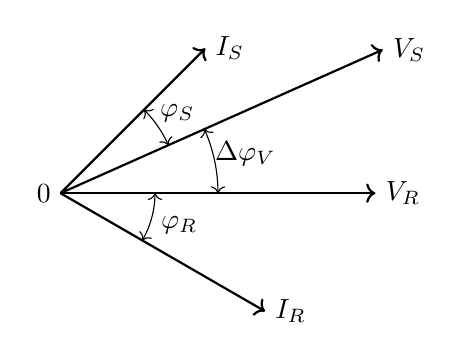
\begin{tikzpicture}
								\coordinate (origo) at (0,0);
								\coordinate (pivot) at (1,5);
    
    							\draw (0,0) node[left] {$0$};
    							\draw[thick,->] (origo) -- ++(4,0) node (VR) [right] {$V_R$};

								\draw[thick,->] (origo) -- ++(330:3) coordinate (IR) node[right] {$I_R$};
								
								\draw[thick,->] (origo) -- ++(405:2.6) coordinate (IS) node[right] {$I_S$};
    
							    \draw[thick,->] (origo) -- ++(384:4.48) coordinate (VS) node[right] {$V_S$};

								\pic [draw, <->, "$\varphi_R$", angle eccentricity=1.3, angle radius=1.2cm] {angle = IR--origo--VR};
    
								\pic [draw, <->, "$\varphi_S$", angle eccentricity=1.2, angle radius=1.5cm] {angle = VS--origo--IS};
    
							    \pic [draw, <->, "$\Delta \varphi_V$", angle eccentricity=1.2, angle radius=2cm] {angle = VR--origo--VS};
							\end{tikzpicture} \hspace{1cm}							
							 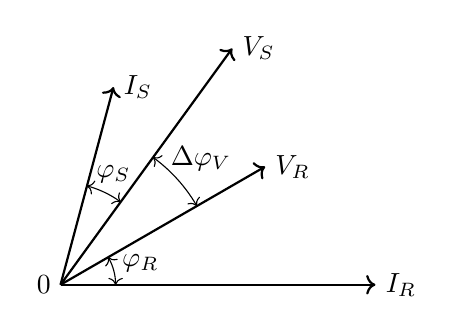
\begin{tikzpicture}
    							\coordinate (origo) at (0,0);
   								\coordinate (pivot) at (1,5);
    
    							\draw (0,0) node[left] {$0$};
							    \draw[thick,->] (origo) -- ++(4,0) node (IR) [right] {$I_R$};

								\draw[thick,->] (origo) -- ++(435:2.6) coordinate (IS) node[right] {$I_S$};
								
							    \draw[thick,->] (origo) -- ++(390:3) coordinate (VR) node[right] {$V_R$};
    
							    \draw[thick,->] (origo) -- ++(414:3.71) coordinate (VS) node[right] {$V_S$};

							    \pic [draw, <->, "$\varphi_R$", angle eccentricity=1.5, angle radius=.7cm] {angle = IR--origo--VR};
    
							    \pic [draw, <->, "$\varphi_S$", angle eccentricity=1.2, angle radius=1.3cm] {angle = VS--origo--IS};
    
								\pic [draw, <->, "$\Delta \varphi_V$", angle eccentricity=1.2, angle radius=2cm] {angle = VR--origo--VS};
						  \end{tikzpicture}
						\end{center}
						\caption{Giản đồ vector cho bài tập \ref{Ex-tham-so-duong-day:bt3}} \label{Fig:gian-do-vector-bt3}
					\end{figure}
			\end{enumerate}
	\end{enumerate} 						% Các tham số của đường dây truyền tải trên không
\addcontentsline{toc}{section}{Tài liệu tham khảo}
\section*{Tài liệu tham khảo}
\begin{enumerate}[{[1.]}]
	\item Nguyễn Hoàng Việt -- Hồ Văn Hiến -- Phan Thị Thanh Bình -- Võ Văn Huy Hoàng, \emph{Thiết kế hệ thống điện}, Tái bản lần thứ hai, NXB ĐHQG TP. Hồ Chí Minh, Năm 2004.
	
	\item Hồ Văn Hiến, \emph{Hệ thống điện Truyền tải và Phân Phối}, Tái bản lần thứ nhất, NXB ĐHQG TP. Hồ Chí Minh, Năm 2005.
\end{enumerate} 															% Tài liệu tham khảo
\end{document}